% NeurIPS 2026 Submission
\documentclass{article}

% NeurIPS style -- [preprint] for a clean one-column draft, [final] for camera-ready.
\usepackage[preprint,nonatbib]{neurips_2026}

\PassOptionsToPackage{table}{xcolor}
\usepackage[utf8]{inputenc}
\usepackage[T1]{fontenc}
\usepackage[breaklinks,colorlinks]{hyperref}
\usepackage{url}
\usepackage{booktabs}
\usepackage{amsmath}
\usepackage{amsfonts}
\usepackage{amssymb}
\usepackage{nicefrac}
\usepackage{microtype}
\usepackage{graphicx}
\usepackage{multirow}
\usepackage{tabularx}
\usepackage{xcolor}
\usepackage{colortbl}
\usepackage{subcaption}
\usepackage{float}
\usepackage{placeins}

\newcounter{algorithm}
\newenvironment{cvpralgorithm}{\begin{figure}[tbp]\refstepcounter{algorithm}\noindent\begin{minipage}{\linewidth}}{\end{minipage}\end{figure}}
\newcommand{\algorithmcaption}[1]{\noindent\emph{Algorithm \thealgorithm. #1}\par\vspace{2pt}}
\newcommand{\algkw}[1]{\emph{#1}}
\newcommand{\algindent}{\hspace*{1.2em}}
\newcommand{\algindenttwo}{\hspace*{2.4em}}
\newcommand{\etal}{\emph{et al.}}

\title{Depth-Conditioned Pseudo-Labels for \\ Scene-Centric Unsupervised Panoptic Segmentation}

\author{Anonymous Author(s)}

\begin{document}
\raggedbottom

\maketitle

\begin{abstract}
Existing unsupervised panoptic methods for full driving scenes rely on calibrated stereo and unsupervised optical flow, which excludes the long tail of monocular footage from phones, dashcams, and fixed cameras. The cues that stereo and motion provided---redundancy across complementary signals---are recoverable from agreement among single-frame priors. On this principle we introduce two compact mechanisms. DCFA is a residual adapter with around 225K parameters that conditions a frozen unsupervised semantic code on monocular depth. SIMCF is a learning-free filter that enforces semantic, geometric, and appearance agreement on candidate panoptic labels. Trained on raw monocular pseudo-labels, the adopted CUPS~\cite{hahn2025cups} panoptic trainer already reaches 32.76 PQ on Cityscapes val under matched evaluation; adding DCFA and SIMCF lifts the same trainer to 35.83 PQ, a contribution-isolated $+$3.07 PQ over the matched monocular baseline. The +5.0 PQ gap between the monocular baseline (32.76) and the published CUPS stereo+flow configuration (27.80~\cite{hahn2025cups}) reflects the change in pseudo-label source and is not attributable to DCFA or SIMCF.
\end{abstract}

%=========================================================================
\section{Introduction}
\label{sec:intro}
%=========================================================================

Most driving footage that ingests into perception pipelines---phone video, dashcam captures, fixed-camera streams---is monocular. Supervised panoptic segmentation dominates benchmarks but requires dense per-instance annotation that does not scale across datasets and domains. The unsupervised setting asks whether panoptic structure can be recovered from raw pixels alone, and current scene-centric methods answer this only when stereo and motion cues are available at pseudo-label time.

Three recent lineages partially answer this. Self-supervised semantic discovery on top of frozen DINO/DINOv2 features~\cite{caron2021dino,oquab2024dinov2} yields region-level partitions usable as semantic pseudo-labels~\cite{hamilton2022stego,kim2024cause}; cut-and-learn instance discovery~\cite{simeoni2021lost,wang2023tokencut,wang2023cutler} extracts foreground masks and bootstraps class-agnostic detectors; CutS3D~\cite{sick2025cuts3d} adds 3-D depth-graph cuts for scene-centric instance separation. CUPS~\cite{hahn2025cups}, the current scene-centric state of the art, combines semantic pseudo-labels with stereo-derived depth and unsupervised scene flow, then trains a Cascade Mask R-CNN with DropLoss bootstrapping and EMA self-training. The stereo and motion cues at pseudo-label time, however, are unavailable for the long tail of monocular footage from phones, dashcams, and fixed cameras --- which narrows the imagery to which unsupervised panoptic segmentation can be applied.

We show that frozen monocular priors are sufficient when composed through cross-modal agreement. Semantic codes provide class-consistent regions but can merge adjacent same-class objects or split surfaces under illumination change; monocular depth exposes physical separations but over-fragments along material seams; dense feature similarity merges depth fragments whose appearance is compatible. Our pipeline uses these cues conservatively: depth proposes candidate boundaries, while semantic identity and feature similarity decide which boundaries survive. Our contributions are twofold. First, we show that frozen monocular priors, composed through cross-modal agreement, are sufficient to seed scene-centric panoptic pseudo-label generation, removing the calibrated stereo and unsupervised optical flow inputs that CUPS~\cite{hahn2025cups} relies on at pseudo-label time. Second, we propose two compact mechanisms that realise this composition: DCFA, a $\sim$225K-parameter residual adapter that conditions a frozen unsupervised semantic code on monocular depth, and SIMCF, a learning-free filter that enforces semantic, geometric, and appearance agreement on candidate panoptic labels. We validate the resulting pipeline on Cityscapes~\cite{cordts2016cityscapes} under the CUPS~\cite{hahn2025cups} evaluation protocol and on cross-dataset transfer to KITTI~\cite{geiger2012kitti}, Waymo V2~\cite{sun2020waymo}, and Mapillary Vistas v2~\cite{neuhold2017mapillary} (Section~\ref{sec:experiments}).

\begin{figure}[tbp]
\centering
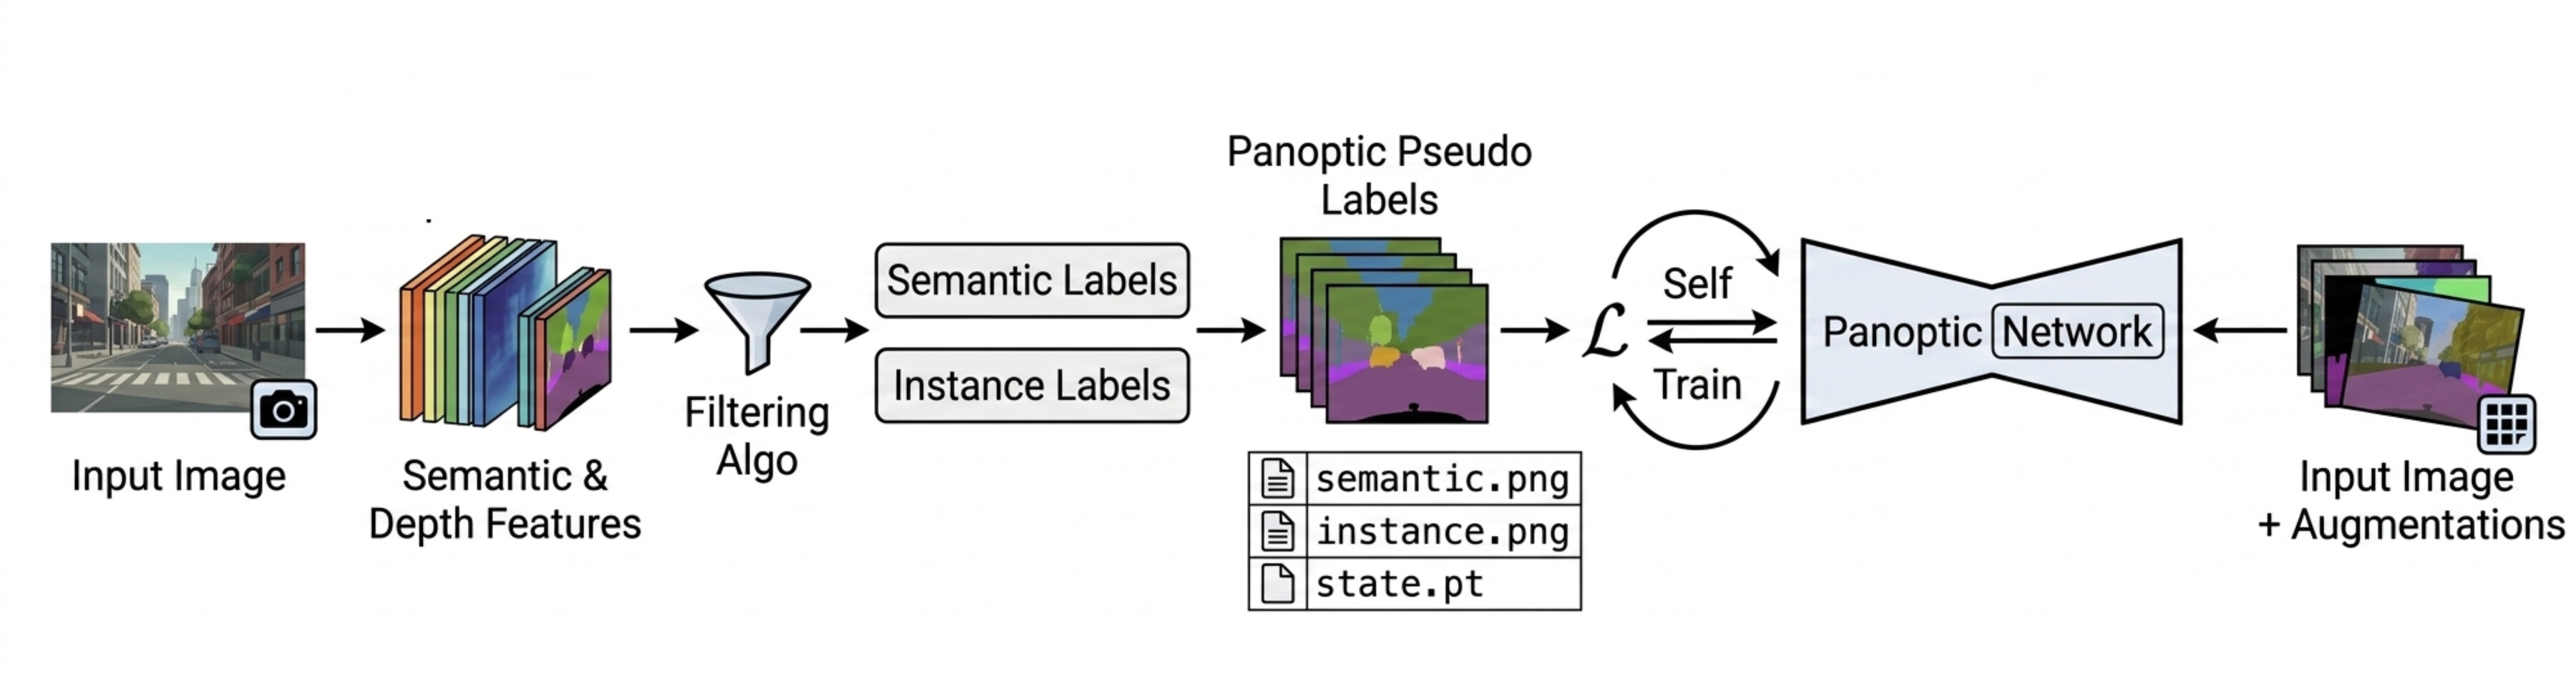
\includegraphics[width=\textwidth]{figures/pipeline_overview.jpg}
\caption{Pipeline overview. Stage 1 constructs panoptic pseudo-labels from a single RGB image using frozen semantic features, monocular depth, DCFA, and SIMCF. Stage 2 adopts CUPS-style~\cite{hahn2025cups} panoptic bootstrapping and panoptic network training on the filtered labels.}
\label{fig:pipeline_overview}
\end{figure}

%=========================================================================
\FloatBarrier
\section{Related Work}
\label{sec:related}
%=========================================================================

\paragraph{Unsupervised Semantic Segmentation with Depth.}
Unsupervised semantic segmentation has migrated from clustering-based objectives~\cite{ji2019iic,cho2021picie} to distillation on top of self-supervised ViT features~\cite{caron2021dino,oquab2024dinov2}, with STEGO~\cite{hamilton2022stego}, HP~\cite{seong2023hp}, and CAUSE~\cite{kim2024cause} producing dense semantic codes; recent refinements~\cite{kim2024eagle,seong2024ppap,couairon2024diffcut,bonnet2024hierarchy} sharpen the clustering objective without changing the substrate. Monocular depth has been used as an auxiliary signal in DepthG~\cite{sick2024depthg}, in CUPS~\cite{hahn2025cups}, and as multi-task pretraining~\cite{hoyer2021threeways}; supervised RGB-D fusion~\cite{yin2025dformerv2} requires dense labels. DCFA differs along two axes: \emph{conditioning site} (a feature-level residual adapter on a frozen clusterbook code, $\sim$225K trainable parameters, vs.\ end-to-end backbone updates in DepthG) and \emph{what is conditioned} (an already-trained, frozen unsupervised code, preserved on its original manifold). To our knowledge, DCFA is the first feature-level residual adapter applied to a frozen unsupervised concept-clusterbook code for monocular depth conditioning.

\paragraph{Unsupervised Instance Segmentation.}
The dominant line applies graph-cut-style partitioning to self-supervised features: LOST~\cite{simeoni2021lost}, TokenCut~\cite{wang2023tokencut}, MaskCut and CutLER~\cite{wang2023cutler}, MaskDistill~\cite{vangansbeke2022maskdistill}, and FreeSOLO~\cite{wang2022freesolo} establish the cut-and-learn template. Recent extensions diversify it with multi-SSL voting (CuVLER~\cite{arica2024cuvler}), single-pass cutting (COLER~\cite{feng2025coler}), prompt-and-merge (ProMerge~\cite{li2024promerge}), boundary-field learning (unMORE~\cite{yang2025unmore}), granularity-controlled SA-1B-scale segmentation (UnSAM/UnSAMv2~\cite{wang2024unsam,yu2025unsamv2}), and slot-attention object discovery (DINOSAUR~\cite{seitzer2023dinosaur}, MR-DINOSAUR~\cite{gong2025mrdinosaur}). The closest comparison to our instance pipeline is CutS3D~\cite{sick2025cuts3d}, which lifts depth to a 3-D point cloud and applies LocalCut on a 3-D k-NN graph. We share CutS3D's monocular premise but stay entirely in 2-D: depth gradients provide a 2-D proxy for the same physical-separation cue, supplied via Sobel filtering and connected-component analysis within thing-eligible semantic regions, without lifting to a 3-D graph.

\paragraph{Unsupervised Panoptic Segmentation.}
Three works frame the current scene-centric Cityscapes~\cite{cordts2016cityscapes} literature. U2Seg~\cite{niu2024u2seg} introduced the first unified unsupervised framework for combined semantic and instance segmentation, composing STEGO-style semantic features with MaskCut instance proposals on object-centric pretraining data and transferring the resulting model to scene-centric benchmarks. CUPS~\cite{hahn2025cups} established the current scene-centric state of the art by constructing pseudo-labels from stereo video, unsupervised optical flow~\cite{stone2021smurf}, and SF2SE3 scene-flow segmentation~\cite{sommer2022sf2se3}, then training a Cascade Mask R-CNN with DropLoss bootstrapping followed by three rounds of EMA self-training. S2-UniSeg~\cite{xu2025s2uniseg} proposed a single-stage monocular alternative based on segmentation-oriented pretraining at the SA-1B scale ($\sim$11M images) followed by adaptation to the target dataset, removing the multi-stage pseudo-label pipeline at the cost of a larger pretraining corpus.


%=========================================================================
\section{Method}
\label{sec:method}
%=========================================================================

\subsection{Problem Setup and Pipeline Overview}
\label{sec:method:setup}

We address scene-centric unsupervised panoptic segmentation in the monocular variant of the CUPS setting~\cite{hahn2025cups}, where a model must produce dense panoptic predictions without human annotations. Concretely, training is given an unlabeled image set $\mathcal{D}_{\text{train}} = \{x_i\}_{i=1}^{N}$, in which each frame $x_i \in \mathbb{R}^{H \times W \times 3}$ is a single RGB image drawn from the target dataset, here Cityscapes~\cite{cordts2016cityscapes}. The setting provides no semantic, instance, or panoptic annotations, no ground-truth or sensor-provided depth maps, no calibrated stereo views, and no temporal neighbours. We use only unlabeled target images for pseudo-label construction and panoptic network training, while relying on frozen off-the-shelf visual and depth priors. Formally, the two stages can be written as
\begin{equation}
G(x) = (\hat S_x, \hat I_x), \qquad F(x) = (S_x, I_x),
\label{eq:pipeline}
\end{equation}
where $G$ is the monocular pseudo-label generator used during training and $F$ is the panoptic network evaluated at test time. The maps $\hat S_x$ and $S_x$ assign semantic labels to pixels, while $\hat I_x$ and $I_x$ assign instance identities to pixels belonging to countable object classes.

Figure~\ref{fig:pipeline_overview} summarizes the two-stage pipeline. The first stage fits a Stage-1 generator on unlabeled target images and applies it independently to each frame; the second stage follows the panoptic bootstrapping and network-training procedures of CUPS~\cite{hahn2025cups} on the resulting pseudo-labels. Holding the training stage fixed lets us attribute changes in final performance to the pseudo-label source, which is also the only place where stereo and motion cues entered CUPS.

The Stage-1 generator is built from three modules on top of frozen, target-annotation-free priors --- a DINOv2 ViT-B/14 backbone~\cite{oquab2024dinov2} and the CAUSE-TR head~\cite{kim2024cause}. The semantic branch produces $\hat S_x$ by passing $x$ through the frozen backbone and CAUSE-TR head to obtain a 90-dimensional code, refined by the Depth-Conditioned Feature Adapter (DCFA) before clustering. The instance branch produces $\hat I_x$ from Sobel responses on a monocular depth map, restricted to thing-eligible semantic regions. SIMCF then filters the candidate labels by checking semantic identity, instance geometry, and feature similarity.


\subsection{Monocular Pseudo-Label Baseline}
\label{sec:method:baseline}

\begin{figure}[tbp]
\centering
\begin{subfigure}{\textwidth}
\centering
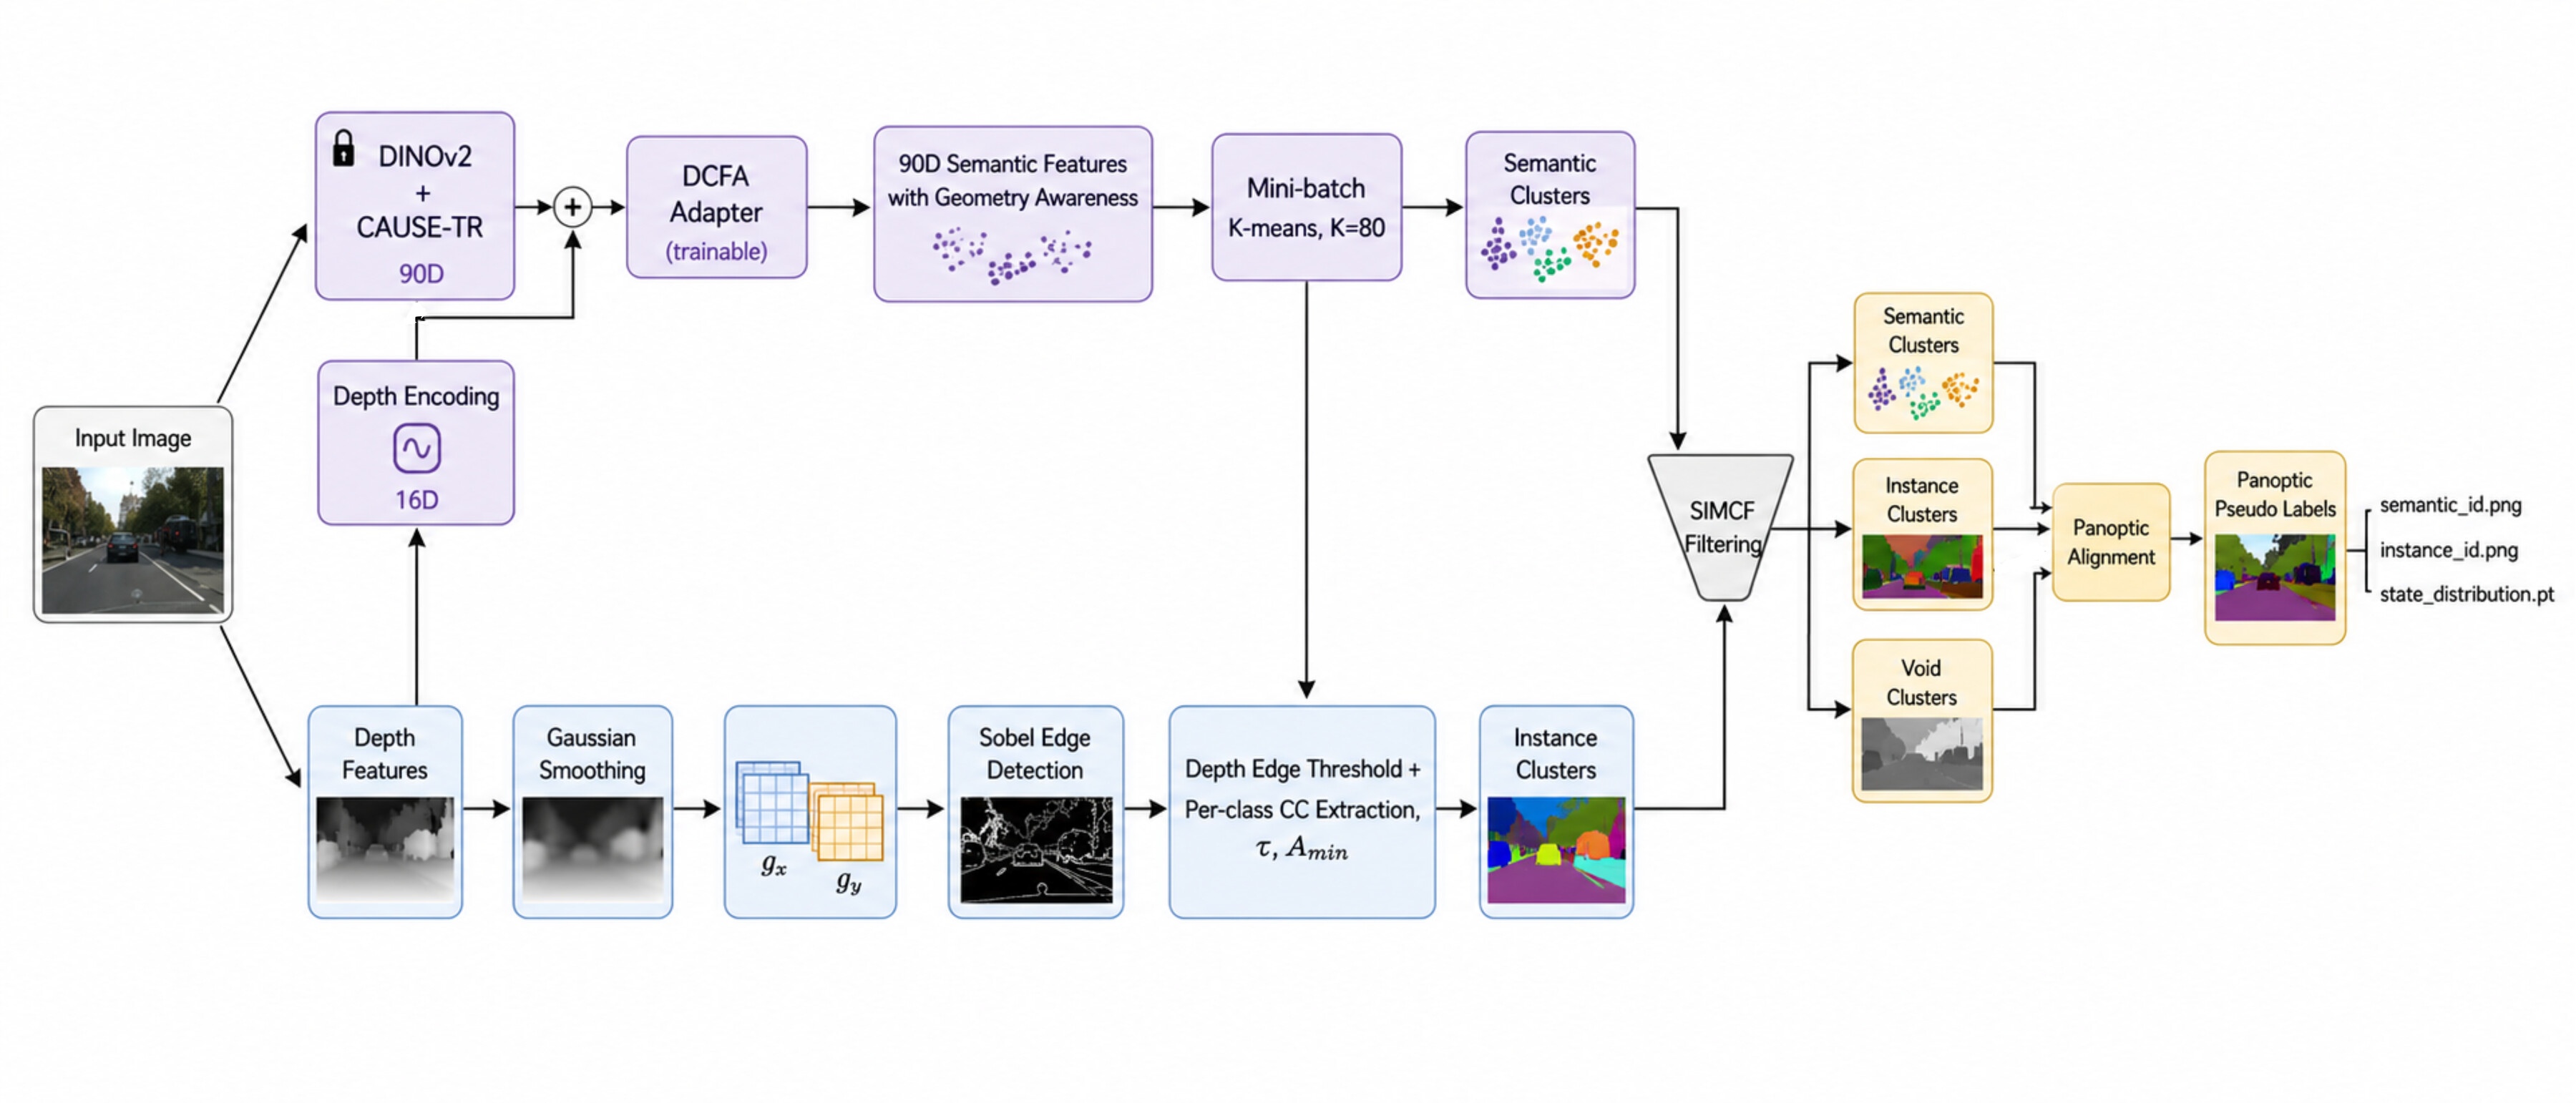
\includegraphics[width=\textwidth]{figures/pseudo_label_generation.jpg}
\caption{Pseudo-label generation. The semantic branch clusters depth-conditioned CAUSE-TR~\cite{kim2024cause} codes; the instance branch converts monocular depth gradients into connected components inside thing-eligible regions; SIMCF filters candidate labels.}
\label{fig:pseudolabel_generation}
\end{subfigure}\\[2pt]
\begin{subfigure}{0.7\linewidth}
\centering

\includegraphics[width=\linewidth]{figures/dcfa_adapter_training.png}
\caption{DCFA adapter training. A frozen CAUSE-TR code is adjusted by a depth-conditioned residual before $k$-means clustering, with a preservation term keeping the adapted code on the original frozen semantic manifold.}
\label{fig:dcfa_adapter}
\end{subfigure}
\caption{Stage-1 pipeline. (a) End-to-end pseudo-label generation. (b) DCFA adapter training detail.}
\label{fig:stage1}
\end{figure}

Stereo and scene flow give CUPS~\cite{hahn2025cups} access to physical-separation cues at pseudo-label time: a 3-D boundary between two adjacent surfaces produces a discontinuity in disparity or in inter-frame motion that separates one instance from another. Monocular depth exposes many of the same physical-separation cues in a single frame, provided that the discontinuity is read at the right spatial scale and only within a region whose semantic identity has already been estimated. Figure~\ref{fig:stage1}(a) shows how the semantic and depth branches provide the raw candidate labels that SIMCF later filters.

The semantic branch is assembled entirely from frozen priors. Each image $x$ is encoded by a frozen DINOv2 ViT-B/14 backbone~\cite{oquab2024dinov2}, whose dense patch features are then reduced by a frozen CAUSE-TR head~\cite{kim2024cause} to a 90-dimensional semantic code. We L2-normalize these codes and partition them with k-means on the unlabeled training set into $k = 80$ centroids, assigning each pixel the index of its nearest centroid to obtain $\hat S_x$. The cardinality $k = 80$ is deliberately well above the 27-class evaluation taxonomy: collapsing to 27 classes at this stage would erase fine visual modes that the depth-based instance branch later relies on. CUPS reports that this regime monotonically improves panoptic quality as $k$ exceeds the evaluation cardinality~\cite{hahn2025cups}.

With $\hat S_x$ in hand, the instance branch reads physical-separation structure from a single monocular depth map $D \in \mathbb{R}^{H \times W}$. We use a frozen DepthPro network~\cite{bochkovskii2024depthpro}, chosen because it balances boundary sharpness against surface smoothness. We apply $3 \times 3$ Sobel kernels $K_x, K_y$ to $D$ and flag candidate boundaries by thresholding the resulting gradient magnitude,
\begin{equation}
\begin{aligned}
g_D(p) &= \sqrt{(K_x * D)^2(p) + (K_y * D)^2(p)}, \\
B_D(p) &= \mathbf{1}\{g_D(p) > \tau_d\}, \qquad \tau_d = 0.20 .
\end{aligned}
\label{eq:depth_boundary}
\end{equation}
Pixels with $B_D(p)=1$ are flagged as candidate boundaries. We set $\tau_d = 0.20$ using label-free pseudo-instance statistics; sharper thresholds over-fragment the training data, as discussed alongside Table~\ref{tab:depth}. Connected-component labelling with 8-neighbour adjacency is run only inside thing-eligible semantic regions. Each of the 80 over-clusters is assigned to its nearest concept in the CAUSE~\cite{kim2024cause} 27-class self-supervised vocabulary by centroid distance in the 90-dimensional code space, and thing-eligibility is read off the CAUSE taxonomy~\cite{kim2024cause} (eight countable categories). This over-cluster-to-concept map $\phi$ is computed entirely from frozen self-supervised features and uses no ground-truth labels; a precise specification is given in Appendix~\ref{sec:supp:impl:phi}. Components below $A_\text{min} = 1000$ pixels are discarded, and the surviving components are dilated with three iterations of a $3 \times 3$ structuring element.

The semantic regions inherited from the frozen CAUSE-TR~\cite{kim2024cause} code are appearance-driven and can split a single physical surface across an illumination change or merge two adjacent same-class objects. Closing this gap requires conditioning the semantic code on the same depth signal that already governs the instance branch.


\subsection{Depth-Conditioned Feature Adapter (DCFA)}
\label{sec:method:dcfa}

Figure~\ref{fig:stage1}(b) summarizes the adapter path. We introduce a small residual adapter that consumes the depth value $d_u$ at pixel $u$ and adds a learned depth-driven shift to the frozen 90-dimensional code $z_u$, nudging cluster boundaries toward depth-consistent regions where appearance fails.

Conditioning on $d_u$ requires a representation rich enough for a small MLP to read both fine boundary differences and coarse depth ordering. Since $d_u \in [0, 1]$ is a scalar, we lift it through a 16-dimensional sinusoidal positional encoding with eight exponentially-spaced frequencies $\omega_k = 2^k \pi$ for $k = 0, \dots, 7$,
\begin{equation}
\begin{aligned}
e(d_u) = \big[ &\sin(\omega_0 d_u), \cos(\omega_0 d_u), \dots, \\
              &\sin(\omega_7 d_u), \cos(\omega_7 d_u) \big] \in \mathbb{R}^{16}.
\end{aligned}
\label{eq:sinusoid}
\end{equation}
The encoding $e(d_u)$ is concatenated with the frozen code $z_u$ into a 106-dimensional input, which a three-layer MLP $A: \mathbb{R}^{106} \to \mathbb{R}^{90}$ (two 384-wide hidden layers, each with layer normalization and ReLU, and a zero-initialized output projection) maps to a residual shift added to the frozen code,
\begin{equation}
\tilde z_u = z_u + A([z_u,\, e(d_u)]).
\label{eq:residual}
\end{equation}
The construction has approximately 225K (225,114) trainable parameters, small relative to the $\sim$86M parameters of the frozen ViT backbone. Zero initialisation of the output projection makes $\tilde z_u = z_u$ at step 0, so any departure from the frozen code is acquired gradually under the loss below.

Training applies the DepthG~\cite{sick2024depthg} depth-feature correlation loss to the adapted code rather than to the backbone weights, paired with a preservation term that penalises drift from $z_u$ and keeps $\tilde z$ on the original CAUSE-TR~\cite{kim2024cause} manifold. The adapter minimizes
\begin{equation}
\begin{aligned}
\mathcal{L}_\text{DCFA}
&= \mathcal{L}_\text{corr}(\tilde z, D)
 + \lambda_p \mathcal{L}_\text{preserve}(\tilde z, z), \\
\lambda_p &= 20 .
\end{aligned}
\label{eq:dcfa_loss}
\end{equation}
$\mathcal{L}_\text{corr}$ is the DepthG~\cite{sick2024depthg} depth-similarity-weighted feature-correlation loss; $\mathcal{L}_\text{preserve}$ is a per-pixel squared distance between $\tilde z_u$ and the frozen $z_u$. Formal definitions and sampling details are in Appendix~\ref{sec:supp:impl}.
\subsection{SIMCF: Semantic Instance Mutual Consistency Filtering}
\label{sec:method:simcf}

DCFA changes the feature space before clustering, but some errors remain after semantic and instance labels are formed. A depth fragment may cut through a single object, a proposal may contain pixels from multiple pseudo-classes, or a semantic assignment may sit at a depth far from the empirical range of its pseudo-class. SIMCF, short for Semantic Instance Mutual Consistency Filtering, is the final algorithm inside $G$: it takes the raw candidate pair $(S_x^0, I_x^0)$ and returns filtered pseudo-labels $(\hat S_x, \hat I_x)$ by enforcing consistency between semantic identity, instance geometry, feature similarity, and depth statistics.

SIMCF runs three sequential checks. \textbf{(A)} For each instance region, the dominant pseudo-class is identified and within-region pixels of conflicting classes are reassigned, preventing mixed-class instance targets. \textbf{(B)} Adjacent proposal pairs whose mean DINOv3 features~\cite{simeoni2025dinov3} agree above $\tau_\text{sim}$ and whose dominant classes match are merged, repairing depth over-fragmentation. \textbf{(C)} Pixels whose depth lies more than $\eta\sigma_c$ from the per-class depth mean are reassigned to void rather than treated as hard negatives. SIMCF is learning-free; the four hyperparameters $\tau_\text{sim}$, $\eta$, $A_\text{min}$, and 8-neighbour adjacency are fixed across all experiments. A precise specification of the over-cluster-to-concept map $\phi$, including its no-ground-truth construction, is given in Appendix~\ref{sec:supp:impl:phi}.

\begin{figure}[tbp]
\centering
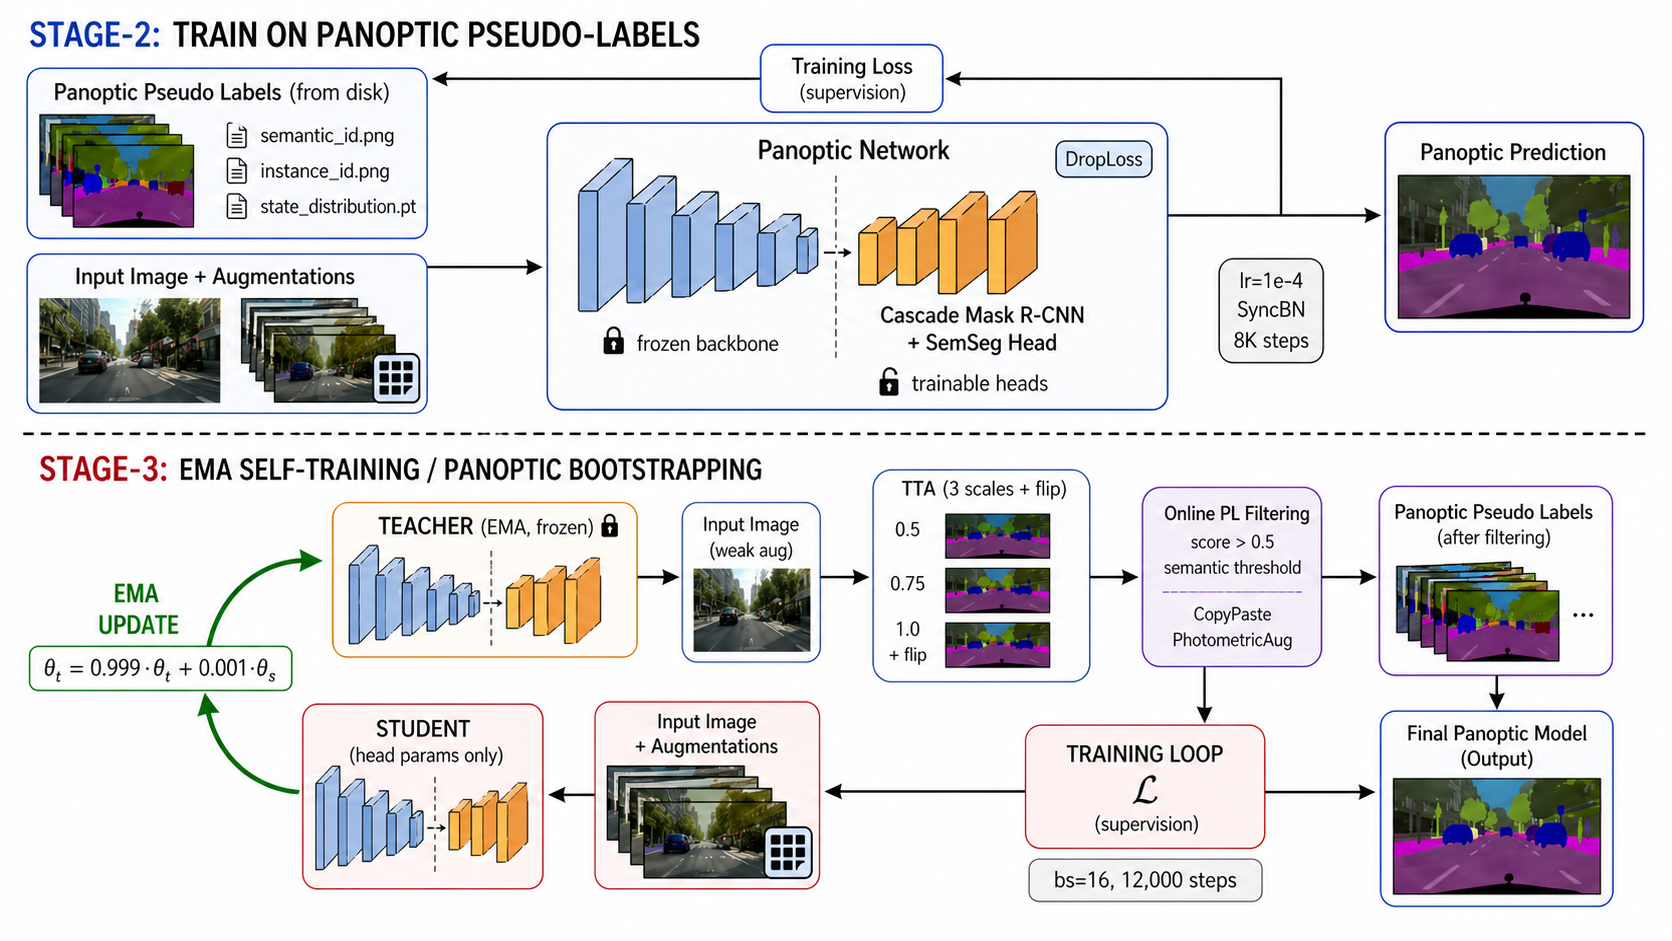
\includegraphics[width=0.90\textwidth]{figures/panoptic_network_training.png}
\caption{Panoptic bootstrapping and panoptic network training. Filtered pseudo-labels supervise the initial panoptic network, and EMA self-training refines the labels and network across subsequent rounds, following the CUPS~\cite{hahn2025cups} training recipe.}
\label{fig:panoptic_training}
\end{figure}

\subsection{Panoptic Bootstrapping and Panoptic Network Training}
\label{sec:method:detector}

Filtering completes the Stage-1 generator $G$. We adopt the panoptic bootstrapping and EMA self-training procedures of CUPS~\cite{hahn2025cups} verbatim --- Cascade Mask R-CNN heads, DropLoss~\cite{wang2023cutler} on void regions, self-enhanced copy-paste augmentation, and three rounds of EMA self-training --- and use the final-round student as the network $F$ in Eq.~\ref{eq:pipeline}. Holding these procedures fixed lets the experiments isolate the effect of the pseudo-label source. Figure~\ref{fig:panoptic_training} shows the training path; full hyperparameters are in Section~\ref{sec:exp:setup} and Appendix~\ref{sec:supp:impl}.

At test time, $F$ produces $(S_x, I_x)$ via the standard panoptic merge~\cite{kirillov2019panoptic}. Two non-obvious design choices: (i) $F$ predicts directly into the pseudo-class vocabulary it was trained on; the Hungarian map to the 27-class Cityscapes~\cite{cordts2016cityscapes} taxonomy is computed only at evaluation time and is the only ground-truth-derived component anywhere in the pipeline. (ii) The thing/stuff partition driving the merge is inherited from the frozen CAUSE-TR~\cite{kim2024cause} taxonomy, so the same partition supervises Stage-1 instance extraction and test-time panoptic merging without taxonomy drift.

%=========================================================================
\FloatBarrier
\section{Experiments}
\label{sec:experiments}
%=========================================================================

We report experiments on Cityscapes~\cite{cordts2016cityscapes} and zero-shot transfer datasets, separating pseudo-label quality from trained-network performance. The evaluation asks whether monocular pseudo-labels can seed the adopted CUPS~\cite{hahn2025cups} training procedure, how much DCFA and SIMCF contribute, and where the fixed Cityscapes-derived pseudo-class vocabulary fails.

\subsection{Experimental Setup}
\label{sec:exp:setup}

Pseudo-label generation and panoptic network training use only Cityscapes train~\cite{cordts2016cityscapes} (2{,}975 images, no annotations); evaluation reports Cityscapes val (500 images) under the 27-class CAUSE~\cite{kim2024cause} pseudo-vocabulary with a Hungarian map to the 27-class Cityscapes label space (\texttt{NUM\_CLASSES=27} in the official CUPS protocol~\cite{hahn2025cups}, the full Cityscapes label space). The Stage-1 generator $G$ couples a frozen DINOv2 ViT-B/14 backbone~\cite{oquab2024dinov2} and CAUSE-TR head~\cite{kim2024cause} with DCFA ($h{=}384$, $\lambda_p{=}20$, $\sim$225K trainable parameters), $k$-means over-clustering at $k{=}80$, the monocular instance branch ($\tau_d{=}0.20$, $A_\text{min}{=}1000$), and SIMCF ($\tau_\text{sim}{=}0.85$, $\eta{=}2.5$); DepthPro~\cite{bochkovskii2024depthpro} supplies the monocular depth map. The panoptic network is a three-stage Cascade Mask R-CNN~\cite{cai2018cascade} on a frozen DINOv3 ViT-B/16 backbone~\cite{simeoni2025dinov3}, trained with CUPS-style~\cite{hahn2025cups} panoptic bootstrapping (8K steps, DropLoss~\cite{wang2023cutler}, copy-paste) followed by three 5K-step EMA self-training rounds. All operating hyperparameters were fixed before consulting Cityscapes annotations; the SIMCF sweep in Appendix~\ref{sec:supp:simcf_sweep} is a retrospective sensitivity analysis, not a model-selection procedure. Full hyperparameter recipes, optimizer schedules, augmentation lists, hardware, and wall-clock budgets are reported in Appendix~\ref{sec:supp:impl} of the supplementary material.


\subsection{Main Cityscapes Results}
\label{sec:exp:main}

Table~\ref{tab:main} records two comparisons on Cityscapes~\cite{cordts2016cityscapes} val: published external references, including CUPS~\cite{hahn2025cups}, and an in-paper controlled comparison that holds the Stage-2/3 trainer fixed. Our method surpasses the published stereo+flow CUPS reference~\cite{hahn2025cups} under its reported evaluation protocol; the per-metric deltas are listed in the bottom row of Table~\ref{tab:main}. The supervised row (62.3 PQ) is an oracle upper bound.

The two ``ours'' rows isolate the contribution of DCFA$+$SIMCF: both share the same Stage-2/3 recipe and Cascade Mask R-CNN backbone; only the Stage-1 pseudo-label source differs. The monocular baseline is trained on raw $K$=80 pseudo-labels (24.54 pseudo-PQ), without DCFA or SIMCF, with Stage-1 inputs differing only in (a) the raw 90-D CAUSE-TR~\cite{kim2024cause} code (no DCFA residual), and (b) DepthPro connected components at $\tau_d = 0.20$ with no SIMCF filtering.

\begin{table}[tbp]
\caption{Unsupervised panoptic segmentation on Cityscapes~\cite{cordts2016cityscapes} val (all in \%, $\uparrow$). ``PL inputs'' are the inputs available at pseudo-label time. ``Eval cls.'' is the number of benchmark classes used by the CUPS~\cite{hahn2025cups} evaluation protocol; our network predicts $K{=}80$ pseudo-classes and is aligned to the 27-class taxonomy only at metric time (Section~\ref{sec:exp:setup}).}
\label{tab:main}
\centering
\small
\setlength{\tabcolsep}{3pt}
\resizebox{\textwidth}{!}{%
\begin{tabular}{l l l c c c c c c}
\toprule
Method & Training data & PL inputs & Eval cls. & PQ & SQ & RQ & PQ$^\text{Th}$ & PQ$^\text{St}$ \\
\midrule
\rowcolor{black!5} Supervised~\cite{kirillov2019panoptic} & CS & dense labels & -- & 62.3 & 81.8 & 75.1 & 62.4 & 62.1 \\
\midrule
DepthG~\cite{sick2024depthg}$+$CutLER~\cite{wang2023cutler} & CS \& ImageNet & RGB mono. & 27 & 16.1 & 45.4 & 21.1 & \phantom{0}3.0 & 25.7 \\
U2Seg~\cite{niu2024u2seg} & COCO \& ImageNet & RGB mono. & 800$+$27 & 18.4 & 55.8 & 22.7 & 10.2 & 24.3 \\
S2-UniSeg~\cite{xu2025s2uniseg} & SA-1B \& CS & RGB mono. & -- & 25.4 & 66.7 & 35.0 & -- & -- \\
CUPS~\cite{hahn2025cups} & CS & RGB$+$stereo$+$flow & 27 & 27.80 & 57.4 & 35.2 & 17.7 & 35.1 \\
\midrule
Monocular baseline (no DCFA/SIMCF) & CS & RGB mono. & 27 & 32.76 & 62.57 & 40.75 & -- & -- \\
\textbf{Ours (DCFA$+$SIMCF)} & CS & RGB mono. & 27 & \textbf{35.83} & \textbf{62.79} & \textbf{43.78} & \textbf{36.26} & \textbf{35.56} \\
\midrule
\textit{vs.\ CUPS~\cite{hahn2025cups}} (prev.\ scene-centric SOTA) & & & & \textcolor{green!50!black}{$+$8.03} & \textcolor{green!50!black}{$+$5.39} & \textcolor{green!50!black}{$+$8.58} & \textcolor{green!50!black}{$+$18.56} & \textcolor{green!50!black}{$+$0.46} \\
\bottomrule
\end{tabular}
}
\end{table}

The improvement over the pseudo-label generator is concentrated in recognition rather than mask quality, indicating that panoptic bootstrapping and EMA self-training principally amplify class recall while preserving the mask geometry already produced by the Stage-1 generator. The trained-model mIoU of 44.56\% is reported under the 19-class semantic-segmentation evaluation taxonomy used historically for unsupervised mIoU comparison.

The aggregate gain is not uniform: large stuff regions and large vehicles combine high SQ with high RQ, while thin structures and rare classes are recognition-limited. The full per-class breakdown is reported in Appendix~\ref{sec:supp:perclass} of the supplementary material and summarized alongside the failure analysis in Section~\ref{sec:exp:generalization}.

\subsection{Ablations}
\label{sec:exp:ablations}

\paragraph{Pipeline progression.}
Table~\ref{tab:progression} traces how PQ accumulates across the four pipeline stages. Stage-1 raw pseudo-labels reach 24.54 PQ; adding our two Stage-1 contributions (DCFA + SIMCF) lifts pseudo-label PQ to 25.85 ($+1.31$). Stage-2 panoptic bootstrapping then trains a Cascade Mask R-CNN on these pseudo-labels and reaches 28.40 PQ, and Stage-3 EMA self-training carries the network to its final \textbf{35.83 PQ} on Cityscapes~\cite{cordts2016cityscapes} val. Two observations follow. First, every stage of the pipeline contributes a meaningful uplift; the largest single jump is the trained-network step, which converts pseudo-label structure into recognition recall. Second, the contribution of DCFA+SIMCF compounds through training: the $+1.31$ PQ Stage-1 advantage grows to $+3.07$ PQ at the trained-network level, indicating that better pseudo-labels are not only better at pseudo-label time but also amplify under the Stage-2/3 procedure.

\begin{table}[tbp]
\caption{Pipeline progression on Cityscapes~\cite{cordts2016cityscapes} val. Each row adds one component to the row above.}
\label{tab:progression}
\centering
\small
\setlength{\tabcolsep}{3pt}
\begin{tabular}{l l c}
\toprule
\# & Pipeline stage & PQ \\
\midrule
1 & Stage-1 pseudo-labels (raw, no DCFA, no SIMCF) & 24.54 \\
2 & \quad $+$ DCFA $+$ SIMCF (our Stage-1 contributions) & 25.85 \\
3 & \quad $+$ Stage-2 panoptic bootstrapping & 28.40 \\
4 & \quad $+$ Stage-3 EMA self-training (final) & \textbf{35.83} \\
\bottomrule
\end{tabular}
\end{table}

\paragraph{Component contribution.}
Table~\ref{tab:components} reports DCFA $\times$ SIMCF at the fixed training-data instance configuration ($\tau_d = 0.20$). All four cells share the same depth instances; only the pre-clustering adapter and the post-instance filter are toggled. The load-bearing observation is the +1.31 PQ jump from Raw $K$=80 (24.54) to Both (25.85), and the +0.58/+0.63 PQ separation between Both and either single component, which is consistent with the two corrections targeting different failure modes (DCFA reshapes the feature space, SIMCF filters the resulting labels) and combining super-additively. The single-component rows DCFA-only (25.22) and SIMCF-only (25.27) are within 0.05 PQ of each other and should not be read as a strict ordering between the two mechanisms; the relevant claim is complementarity, evidenced by the move from either single component to Both.

\begin{table}[tbp]
\caption{Pseudo-label component complementarity at fixed $\tau_d = 0.20$ DepthPro instances. ``Raw $K$=80'' is the no-DCFA, no-SIMCF baseline. mIoU is the Cityscapes~\cite{cordts2016cityscapes} val 19-class semantic-segmentation mIoU; SIMCF filters instance proposals and does not modify the semantic prediction, so the SIMCF-only and DCFA$+$SIMCF rows inherit the mIoU of the underlying semantic code.}
\label{tab:components}
\centering
\small
\setlength{\tabcolsep}{3pt}
\begin{tabular}{l c c c c c c}
\toprule
Variant & DCFA & SIMCF & PQ & SQ & RQ & mIoU \\
\midrule
Raw $K$=80 & -- & -- & 24.54 & 60.0 & 33.6 & 52.69 \\
DCFA only & \checkmark & -- & 25.22 & 61.0 & 34.0 & 55.29 \\
SIMCF only & -- & \checkmark & 25.27 & 57.5 & 34.4 & 52.69 \\
Both & \checkmark & \checkmark & 25.85 & 58.3 & 34.9 & 55.29 \\
\bottomrule
\end{tabular}
\end{table}

\paragraph{SIMCF threshold sensitivity.}
Sweeping the SIMCF thresholds ($\tau_\text{sim}$, $\eta$) by $\pm{\sim}12\%$ around the paper setting yields a 0.71-point PQ band (25.27--25.98), smaller than the $+1.31$ PQ super-additive gap from either single component to Both in Table~\ref{tab:components}. SIMCF's contribution is therefore robust to moderate threshold perturbation rather than tuned-on-test; the full sweep table is reported in Appendix~\ref{sec:supp:simcf_sweep}.

\paragraph{DCFA conditioning mechanism.}
The novelty claim in Section~\ref{sec:related} contrasts DCFA's architectural depth conditioning with DepthG-style~\cite{sick2024depthg} loss-side conditioning. We separate the contribution of the two axes empirically (Table~\ref{tab:conditioning}). \emph{DepthG~\cite{sick2024depthg} (drop-in)} loads the official DepthG checkpoint~\cite{sick2024depthg} (DINO ViT-B/8 + STEGO-style cluster head trained with depth-correlation loss on Cityscapes train, $\dim{=}100$, ZoeDepth) and uses it as a Stage-1 generator under our identical downstream pipeline (k-means $k$=80, DepthPro depth-CC instances, eval). \emph{Loss-side $P(z)$} replaces DCFA's depth-conditioned residual with a learnable projection $P : \mathbb{R}^{90} \to \mathbb{R}^{90}$ ($P(z) = z + \text{MLP}(z)$, 70K parameters, no depth as architectural input) trained on cached CAUSE~\cite{kim2024cause} codes with only the depth-correlation loss $\mathcal{L}_\text{corr}(P(z), D)$. We further isolate the preservation axis with \emph{Loss-side $P(z)$ + preserve}, which adds $\lambda_p \mathcal{L}_\text{preserve}$ ($\lambda_p=20$) to the loss-side objective.

The decomposition reads as follows. Without preservation, both loss-side methods collapse far below the raw baseline (DepthG~\cite{sick2024depthg} drop-in $-11.21$ PQ; loss-side without preserve $-11.92$ PQ), confirming that any unconstrained re-shaping of a frozen unsupervised concept-clusterbook code degrades the embedding structure that downstream $k$-means relies on. Adding preservation rescues most of the structure (loss-side with preserve reaches 23.83 PQ), but is still $-0.71$ PQ below the raw baseline and $-1.39$ PQ below DCFA. The remaining $+1.39$ PQ gap between loss-side+preserve and DCFA, at matched parameter budget and matched preservation strength, is the empirical contribution of \emph{architectural} depth conditioning -- depth as an input to the conditioning network, not just to the loss. The two axes -- architectural input and explicit manifold preservation -- are both required for the $+0.68$ PQ over raw, and neither is a strict substitute for the other.

\begin{table}[tbp]
\caption{Conditioning-mechanism decomposition at the Stage-1 pseudo-label level (Section~\ref{sec:exp:ablations}). All rows share the same downstream pipeline; only how depth enters the model varies.}
\label{tab:conditioning}
\centering
\scriptsize
\setlength{\tabcolsep}{3pt}
\begin{tabular}{@{}l l c c c c@{}}
\toprule
Method & Conditioning & PQ & SQ & RQ & mIoU \\
\midrule
Raw $K$=80 (paper substrate)        & none                  & 24.54 & 60.00 & 33.60 & 52.69 \\
DepthG~\cite{sick2024depthg} (official, ViT-B/8)          & loss, end-to-end      & 13.33 & 33.39 & 18.56 & -- \\
Loss-side $P(z)$ on CAUSE~\cite{kim2024cause}           & loss, no preserve     & 12.62 & 55.35 & 18.95 & -- \\
Loss-side $P(z)$ + preserve         & loss $+$ preserve     & 23.83 & 56.54 & 32.76 & -- \\
DCFA (ours)                         & residual $+$ preserve & \textbf{25.22} & \textbf{61.00} & \textbf{34.00} & \textbf{55.29} \\
\bottomrule
\end{tabular}
\end{table}

\paragraph{Depth model.}
We compared SPIdepth, Depth-Anything v3~\cite{lin2025da3}, and DepthPro~\cite{bochkovskii2024depthpro} at multiple gradient thresholds and selected DepthPro at $\tau_d{=}0.20$ as the training-data configuration: it produces $\sim$22 instances/image rather than the $\sim$57 instances/image (more than half below 1000 pixels) generated by the sharper $\tau_d{=}0.01$ setting. Full depth-source diagnostics are reported in Appendix~\ref{sec:supp:depth}.


\subsection{Generalization and Failure Analysis}
\label{sec:exp:generalization}

\begin{table}[tbp]
\caption{Cross-dataset generalization on driving-scene benchmarks (PQ/SQ/RQ in \%, $\uparrow$). Published baselines from~\cite{hahn2025cups}~Tab.~2. ``--'' marks datasets a baseline does not report. $^{\S}$KITTI 19-class and 27-class are identical (KITTI GT only contains the 19 standard classes); $^{\P}$Waymo via CUPS~\cite{hahn2025cups} Waymo loader; $^{\dagger}$Mapillary via paper-defined remap. Protocol details discussed in Section~\ref{sec:exp:generalization}; OOD sanity checks (MOTS, COCO-Stuff-27) in Appendix~\ref{sec:supp:ood}.}
\label{tab:transfer}
\centering
\footnotesize
\setlength{\tabcolsep}{4pt}
\resizebox{\textwidth}{!}{%
\begin{tabular}{l c c c c c c c c c}
\toprule
\multirow{2}{*}{Method} & \multicolumn{3}{c}{KITTI~\cite{geiger2012kitti}} & \multicolumn{3}{c}{Waymo V2~\cite{sun2020waymo}$^{\P}$} & \multicolumn{3}{c}{Mapillary v2~\cite{neuhold2017mapillary}$^{\dagger}$} \\
\cmidrule(lr){2-4} \cmidrule(lr){5-7} \cmidrule(lr){8-10}
& PQ & SQ & RQ & PQ & SQ & RQ & PQ & SQ & RQ \\
\midrule
\rowcolor{black!5} Supervised~\cite{kirillov2019panoptic} & 31.9 & 71.7 & 40.4 & 31.5 & 70.1 & 40.9 & -- & -- & -- \\
\midrule
DepthG~\cite{sick2024depthg}$+$CutLER~\cite{wang2023cutler} & 11.0 & 34.5 & 13.8 & 13.4 & 37.3 & 17.0 & -- & -- & -- \\
U2Seg~\cite{niu2024u2seg} & 20.6 & 52.9 & 25.2 & 19.8 & 50.8 & 23.4 & -- & -- & -- \\
CUPS~\cite{hahn2025cups} & 25.5 & 58.1 & 32.5 & 26.4 & 60.3 & 33.0 & -- & -- & -- \\
\midrule
\textbf{Ours (DCFA$+$SIMCF), 19-class}$^{\S}$ & \textbf{34.85} & \textbf{62.43} & \textbf{42.91} & \textbf{43.51} & \textbf{76.82} & \textbf{50.54} & \textbf{39.19} & \textbf{74.59} & \textbf{47.74} \\
\textbf{Ours (DCFA$+$SIMCF), 27-class}$^{\S}$ & \textbf{34.85} & \textbf{62.43} & \textbf{42.91} & \textbf{39.93} & \textbf{71.68} & \textbf{46.91} & \textbf{27.79} & \textbf{59.64} & \textbf{35.43} \\
\midrule
\textit{vs.\ CUPS~\cite{hahn2025cups}} & \textcolor{green!50!black}{$+$9.4} & \textcolor{green!50!black}{$+$4.3} & \textcolor{green!50!black}{$+$10.4} & \textcolor{green!50!black}{$+$17.1} & \textcolor{green!50!black}{$+$16.5} & \textcolor{green!50!black}{$+$17.5} & -- & -- & -- \\
\bottomrule
\end{tabular}
}
\end{table}

Our trained network transfers across the driving class space without retraining. KITTI~\cite{geiger2012kitti} reaches 34.85 PQ ($+$9.35 over CUPS~\cite{hahn2025cups}); Waymo V2~\cite{sun2020waymo} reaches 43.51 PQ ($+$17.11 over CUPS); Mapillary v2~\cite{neuhold2017mapillary} reaches 39.19 PQ. We report each dataset under the 19-class CUPS cross-dataset protocol used by CUPS for KITTI~\cite{geiger2012kitti}, and report KITTI~\cite{geiger2012kitti} and Mapillary~\cite{neuhold2017mapillary} again under the 27-class in-domain protocol for paper-internal consistency (Table~\ref{tab:transfer}). KITTI's~\cite{geiger2012kitti} panoptic ground truth contains only the 19 standard Cityscapes~\cite{cordts2016cityscapes} classes, so the two taxonomies yield identical numbers. Mapillary~\cite{neuhold2017mapillary} and Waymo V2~\cite{sun2020waymo} are both protocol-sensitive: 27-class PQ drops to 27.79 on Mapillary~\cite{neuhold2017mapillary} and to 39.93 on Waymo V2~\cite{sun2020waymo} because the eight low-coverage Cityscapes-27 extras enter the average rather than mapping to void. Waymo V2~\cite{sun2020waymo} follows the CUPS Waymo pathway, mapping raw labels to Cityscapes-19 over its 16 supported classes. Out-of-distribution sanity checks on MOTS~\cite{voigtlaender2019mots} and COCO-Stuff-27~\cite{caesar2018coco} are deferred to Appendix~\ref{sec:supp:ood}; COCO-Stuff-27~\cite{caesar2018coco} (7.83 PQ) is dominated by categories absent from the Cityscapes~\cite{cordts2016cityscapes}-derived vocabulary, marking the vocabulary boundary of in-domain training rather than a transfer failure of the architecture.

Per-class failure analysis (twenty active classes, six vocabulary-dead) and the SIMCF merge-step diagnostics (instance count 44$\to$22, median size 5{,}502$\to$14{,}965 px, stuff contamination 50.7\%$\to$28.0\%) are reported in Appendix~\ref{sec:supp:perclass}.


%=========================================================================
\FloatBarrier
\section{Conclusion}
\label{sec:conclusion}
%=========================================================================

We showed that frozen monocular priors, composed by cross-modal agreement, suffice to seed the CUPS training recipe, removing its stereo and flow requirements at pseudo-label time. DCFA conditions a frozen unsupervised semantic code on monocular depth via a $\sim$225K-parameter residual adapter; SIMCF is a learning-free filter that enforces semantic, geometric, and appearance agreement on candidate labels. Their effect compounds through Stage-2/3 training, with per-component complementarity verified in Section~\ref{sec:exp:ablations} and the controlled +3.07 PQ delta isolated in Table~\ref{tab:main}.

\paragraph{Limitations and scope.}
Our conclusions are scoped to Cityscapes~\cite{cordts2016cityscapes}-style driving scenes, where DepthPro~\cite{bochkovskii2024depthpro} depth and frozen DINO-family features~\cite{oquab2024dinov2,simeoni2025dinov3} replace the structure that stereo and motion provided in CUPS. Three limitations follow: (i) six dead classes in the pseudo-vocabulary are effectively absent after Hungarian alignment (Appendix~\ref{sec:supp:perclass}); (ii) the Cityscapes~\cite{cordts2016cityscapes}-derived label space transfers within driving (Table~\ref{tab:transfer}) but fails on object-centric COCO-Stuff-27~\cite{caesar2018coco} (Appendix~\ref{sec:supp:ood}); (iii) closely-spaced pedestrians remain a recognition bottleneck of the depth branch, upstream of DCFA and SIMCF.


%=========================================================================
\begin{thebibliography}{99}
%=========================================================================
\bibitem{cordts2016cityscapes} M.~Cordts, M.~Omran, S.~Ramos, et~al. The Cityscapes dataset for semantic urban scene understanding. \emph{CVPR}, 2016.
\bibitem{voigtlaender2019mots} P.~Voigtlaender, M.~Krause, A.~Osep, et~al. MOTS: Multi-object tracking and segmentation. \emph{CVPR}, 2019.
\bibitem{geiger2012kitti} A.~Geiger, P.~Lenz, R.~Urtasun. Are we ready for autonomous driving? The KITTI vision benchmark suite. \emph{CVPR}, 2012.
\bibitem{sun2020waymo} P.~Sun, H.~Kretzschmar, X.~Dotiwalla, et~al. Scalability in perception for autonomous driving: Waymo Open Dataset. \emph{CVPR}, 2020.
\bibitem{neuhold2017mapillary} G.~Neuhold, T.~Ollmann, S.~Rota~Bul\`o, P.~Kontschieder. The Mapillary Vistas dataset for semantic understanding of street scenes. \emph{ICCV}, 2017.
\bibitem{caesar2018coco} H.~Caesar, J.~Uijlings, V.~Ferrari. COCO-Stuff: Thing and stuff classes in context. \emph{CVPR}, 2018.
\bibitem{kirillov2019panoptic} A.~Kirillov, K.~He, R.~Girshick, et~al. Panoptic segmentation. \emph{CVPR}, 2019.
\bibitem{caron2021dino} M.~Caron, H.~Touvron, I.~Misra, et~al. Emerging properties in self-supervised vision transformers. \emph{ICCV}, 2021.
\bibitem{oquab2024dinov2} M.~Oquab, T.~Darcet, T.~Moutakanni, et~al. DINOv2: Learning robust visual features without supervision. \emph{TMLR}, 2024.
\bibitem{simeoni2025dinov3} O.~Sim\'eoni, et~al. DINOv3. \emph{arXiv preprint arXiv:2508.10104}, 2025.
\bibitem{kim2024cause} J.~Kim, et~al. Causal unsupervised semantic segmentation. \emph{arXiv preprint arXiv:2310.07379}, 2024.
\bibitem{bochkovskii2024depthpro} A.~Bochkovskii, et~al. Depth Pro: Sharp monocular metric depth in less than a second. \emph{arXiv preprint arXiv:2410.02073}, 2024.
\bibitem{yang2024da2} L.~Yang, et~al. Depth Anything V2. \emph{NeurIPS}, 2024.
\bibitem{lin2025da3} D.~Lin, et~al. Depth Anything 3: Recovering the visual space from any views. \emph{arXiv preprint arXiv:2511.10647}, 2025.
\bibitem{cai2018cascade} Z.~Cai, N.~Vasconcelos. Cascade R-CNN: Delving into high quality object detection. \emph{CVPR}, 2018.
\bibitem{wang2023cutler} X.~Wang, et~al. Cut and Learn for unsupervised object detection and instance segmentation. \emph{CVPR}, 2023.
\bibitem{wang2023tokencut} Y.~Wang, et~al. TokenCut: Self-supervised object discovery and instance segmentation. \emph{CVPR}, 2023.
\bibitem{hahn2025cups} A.~Hahn, et~al. Scene-centric unsupervised panoptic segmentation (CUPS). \emph{CVPR}, 2025.
\bibitem{niu2024u2seg} D.~Niu, et~al. Unsupervised universal image segmentation (U2Seg). \emph{CVPR}, 2024.
\bibitem{xu2025s2uniseg} Y.~Xu, et~al. S2-UniSeg: Single-stage unsupervised universal segmentation. \emph{arXiv preprint arXiv:2508.06995}, 2025.
\bibitem{sick2024depthg} N.~Sick, et~al. Unsupervised semantic segmentation through depth-guided feature correlation and sampling. \emph{CVPR}, 2024.
\bibitem{sick2025cuts3d} N.~Sick, et~al. CutS3D: Cutting semantics in 3D for 2D unsupervised instance segmentation. \emph{ICCV}, 2025.
\bibitem{hamilton2022stego} M.~Hamilton, et~al. STEGO: Unsupervised semantic segmentation by distilling feature correspondences. \emph{ICLR}, 2022.
\bibitem{ji2019iic} X.~Ji, et~al. Invariant information clustering for unsupervised image classification and segmentation. \emph{ICCV}, 2019.
\bibitem{cho2021picie} J.~Cho, et~al. PiCIE: Unsupervised semantic segmentation using invariance and equivariance in clustering. \emph{CVPR}, 2021.
\bibitem{seong2023hp} H.~Seong, et~al. Leveraging hidden positives for unsupervised semantic segmentation. \emph{CVPR}, 2023.
\bibitem{kim2024eagle} C.~Kim, et~al. EAGLE: Eigen aggregation learning for object-centric unsupervised semantic segmentation. \emph{CVPR}, 2024.
\bibitem{seong2024ppap} H.~Seong, et~al. Progressive proxy anchor propagation for unsupervised semantic segmentation. \emph{ECCV}, 2024.
\bibitem{couairon2024diffcut} P.~Couairon, et~al. DiffCut: Diffusion-feature partitioning. \emph{NeurIPS}, 2024.
\bibitem{bonnet2024hierarchy} L.~Bonnet, et~al. Recursive hierarchy clustering. \emph{arXiv preprint}, 2024.
\bibitem{hoyer2021threeways} L.~Hoyer, et~al. Three ways to improve semantic segmentation with self-supervised depth estimation. \emph{CVPR}, 2021.
\bibitem{yin2025dformerv2} B.-W.~Yin, et~al. DFormerv2: Geometry Self-Attention for RGBD Semantic Segmentation. \emph{CVPR}, 2025.
\bibitem{simeoni2021lost} O.~Sim\'eoni, et~al. Localizing Objects with Self-Supervised Transformers and No Labels (LOST). \emph{BMVC}, 2021.
\bibitem{vangansbeke2022maskdistill} W.~Van~Gansbeke, et~al. MaskDistill. \emph{ECCV}, 2022.
\bibitem{wang2022freesolo} X.~Wang, et~al. FreeSOLO: Learning to segment objects without annotations. \emph{CVPR}, 2022.
\bibitem{arica2024cuvler} S.~Arica, et~al. CuVLER: Enhanced unsupervised object discoveries through exhaustive self-supervised transformers. \emph{CVPR}, 2024.
\bibitem{feng2025coler} Y.~Feng, et~al. COLER: Cluster-once unsupervised instance segmentation. \emph{arXiv preprint}, 2025.
\bibitem{li2024promerge} X.~Li, et~al. ProMerge: Prompt and merge for unsupervised instance segmentation. \emph{ECCV}, 2024.
\bibitem{yang2025unmore} L.~Yang, et~al. unMORE: Unsupervised multi-object detection and segmentation through existence and boundary fields. \emph{ICML}, 2025.
\bibitem{wang2024unsam} X.~Wang, et~al. UnSAM: Segment anything without supervision. \emph{NeurIPS}, 2024.
\bibitem{yu2025unsamv2} J.~Yu, et~al. UnSAMv2: Self-supervised learning enables segment anything at any granularity. \emph{arXiv preprint}, 2025.
\bibitem{seitzer2023dinosaur} M.~Seitzer, et~al. DINOSAUR: Bridging the gap to real-world object-centric learning. \emph{ICLR}, 2023.
\bibitem{gong2025mrdinosaur} S.~Gong, et~al. MR-DINOSAUR: Motion-refined object-centric learning. \emph{ICCV Workshops}, 2025.
\bibitem{stone2021smurf} A.~Stone, et~al. SMURF: Self-teaching multi-frame unsupervised RAFT with full-image warping. \emph{CVPR}, 2021.
\bibitem{sommer2022sf2se3} L.~Sommer, et~al. SF2SE3: Clustering scene flow into SE(3)-motions via proposal and selection. \emph{GCPR}, 2022.
\end{thebibliography}

%=========================================================================
% APPENDIX (supplementary material)
%=========================================================================
\clearpage
\appendix
\renewcommand{\thefigure}{\Alph{section}.\arabic{figure}}
\renewcommand{\thetable}{\Alph{section}.\arabic{table}}
% Override default bold paragraph headings with italic in the appendix
\makeatletter
\renewcommand{\paragraph}[1]{\par\smallskip\noindent\textit{#1}\hspace{0.5em}\ignorespaces}
\makeatother

%=========================================================================
\section{Additional Qualitative Figures}
\label{sec:supp:qualitative}
%=========================================================================

\subsection{Stage-1 Pseudo-Label Trace}
\label{sec:supp:stage1_trace}

Figure~\ref{fig:supp_real_data_flow} traces the Stage-1 data flow on real Cityscapes images, showing intermediate pseudo-label outputs together with the paired RGB/label transformations used by panoptic bootstrapping and panoptic network training.

\begin{figure}[H]
\centering
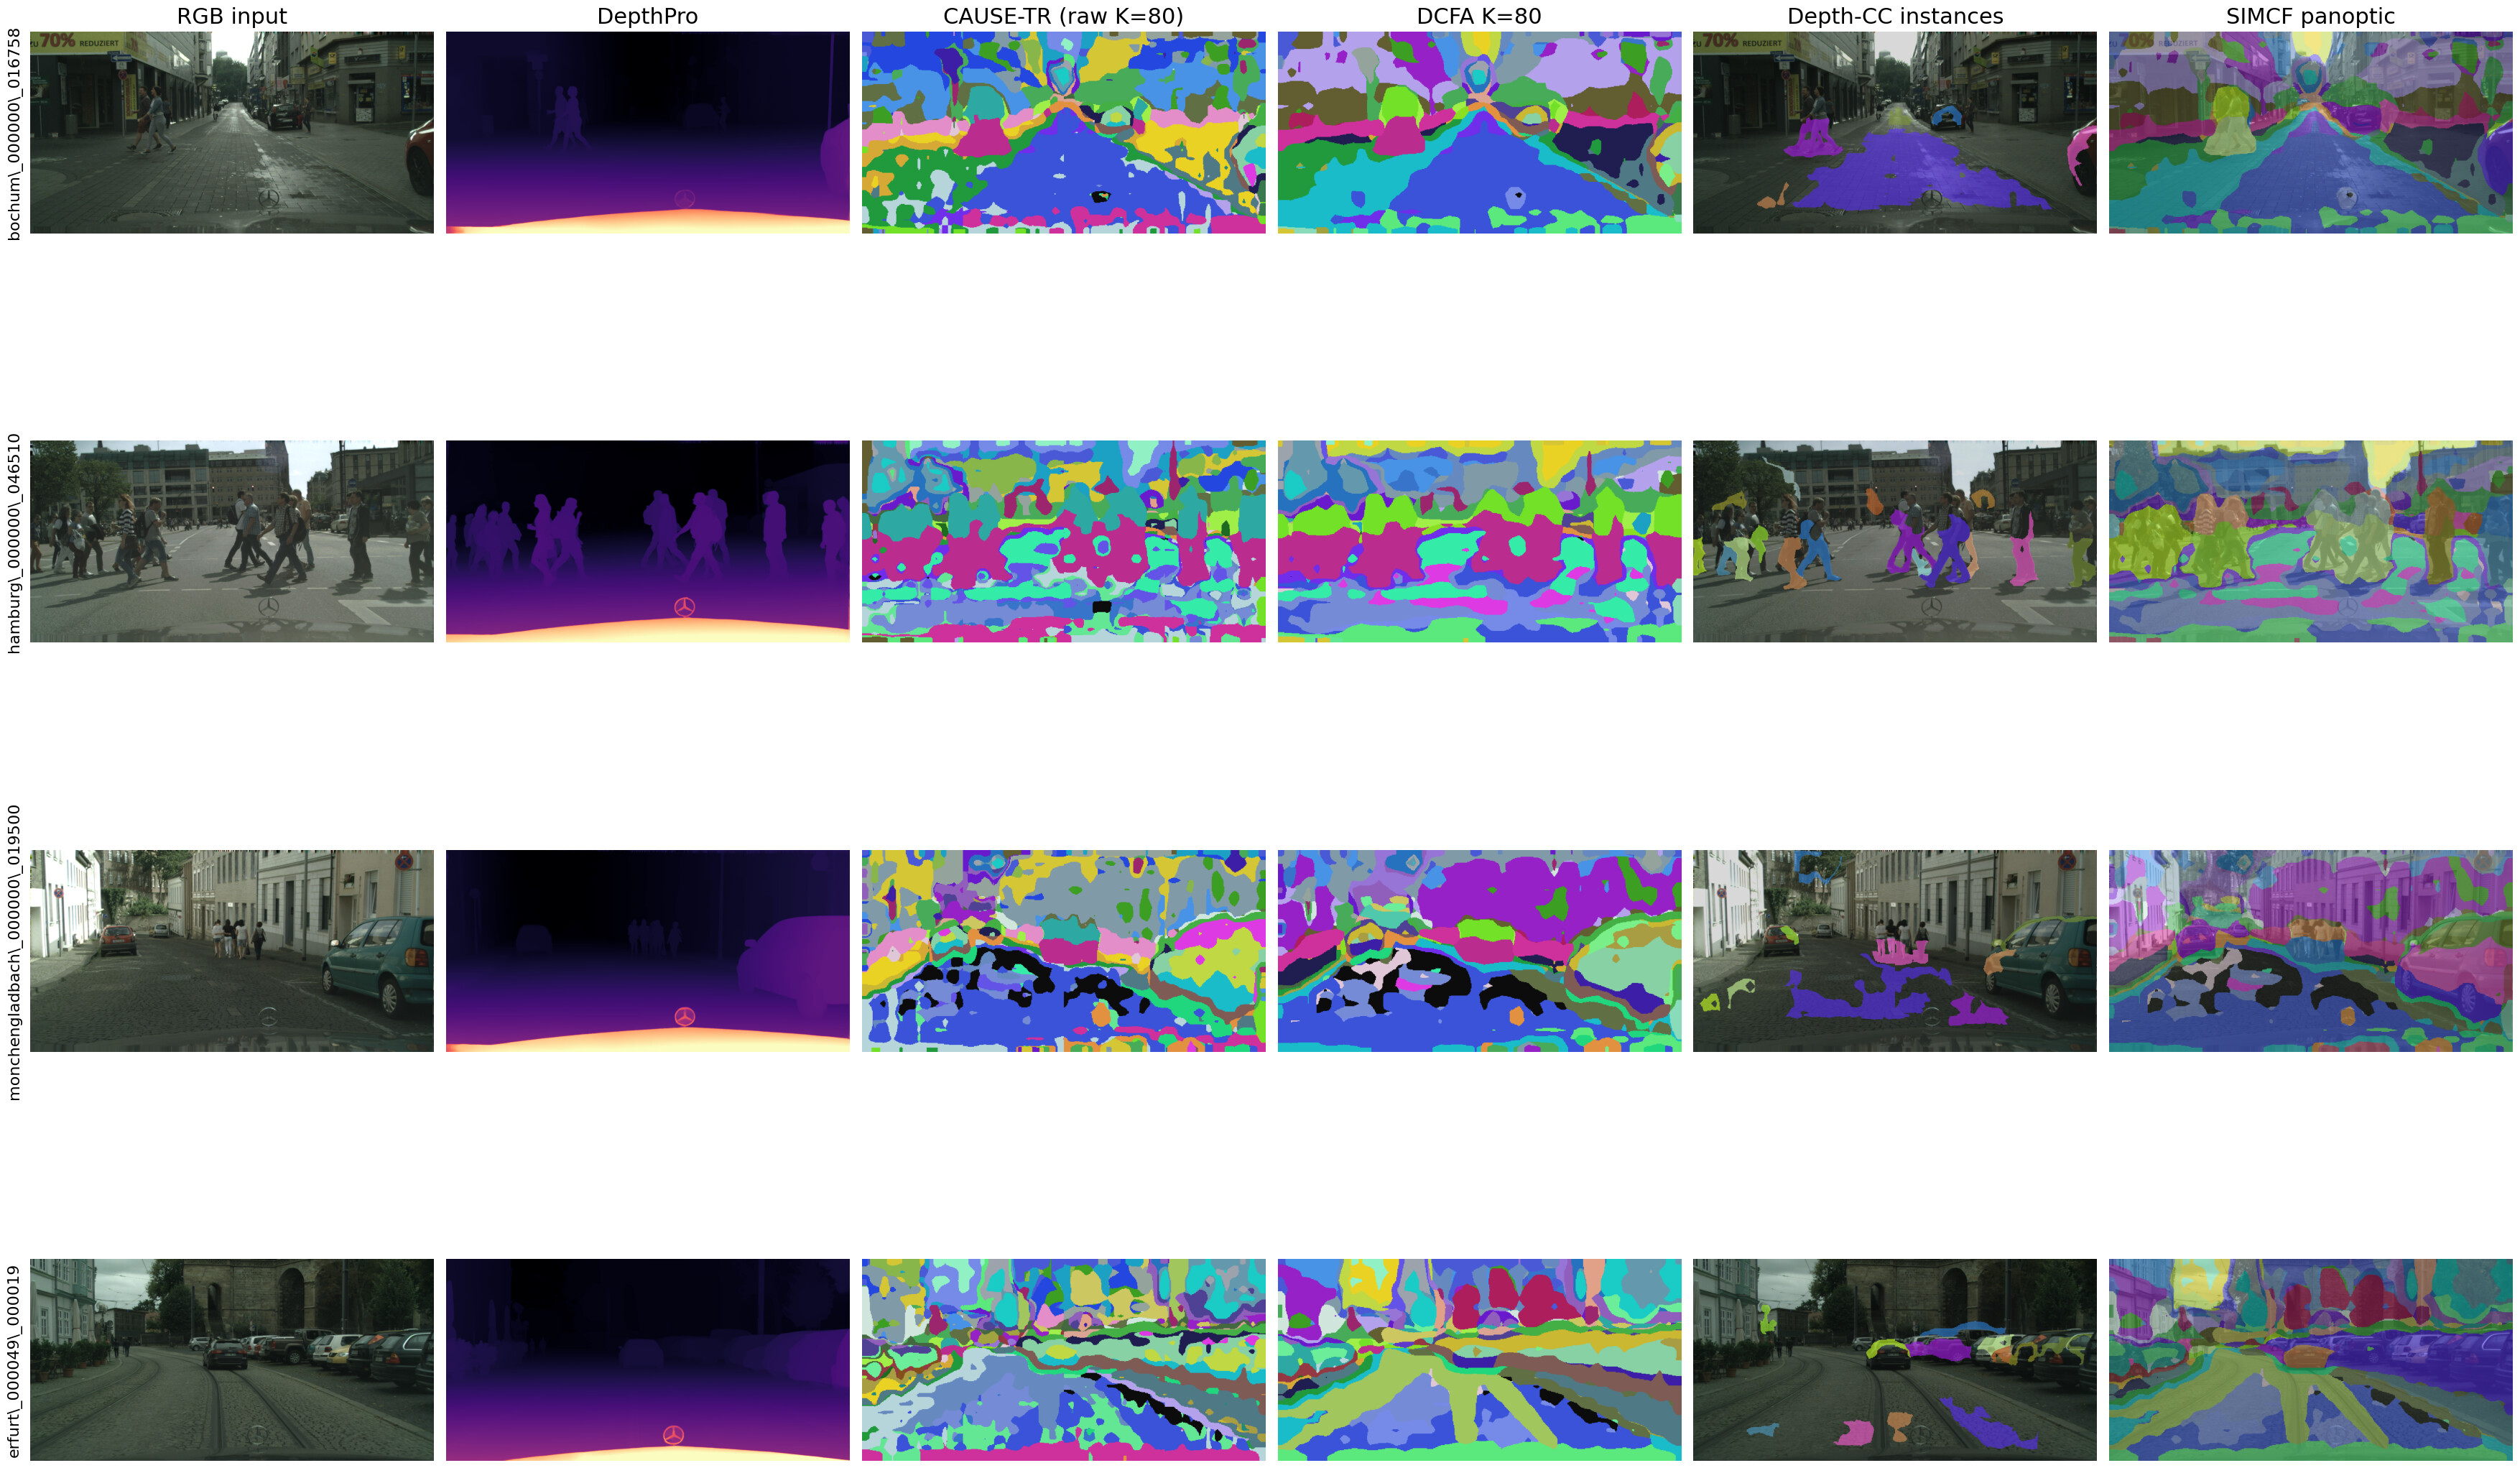
\includegraphics[width=\textwidth]{figures/fig5_stage1_trace_composite.jpg}
\caption{Stage-1 pseudo-label trace on four Cityscapes train frames. Columns: RGB; DepthPro depth; CAUSE-TR~\cite{kim2024cause} raw $K{=}80$ clusters; DCFA-adjusted $K{=}80$; depth-CC instances on RGB; final SIMCF-filtered panoptic pseudo-labels on RGB. Row 2 (hamburg) is the canonical co-planar pedestrian failure case discussed in the main paper's Conclusion section.}
\label{fig:supp_real_data_flow}
\end{figure}

\clearpage

\subsection{Stage-3 Panoptic Predictions}
\label{sec:supp:stage3_predictions}

Figure~\ref{fig:supp_qualitative_stage3} shows representative panoptic predictions from the trained Stage-3 network on nine Cityscapes val images, none of which were used for training. Each row presents the input RGB, the panoptic prediction colorized in the $K=80$ pseudo-class space, and the prediction overlaid on the input.

\begin{figure}[H]
\centering
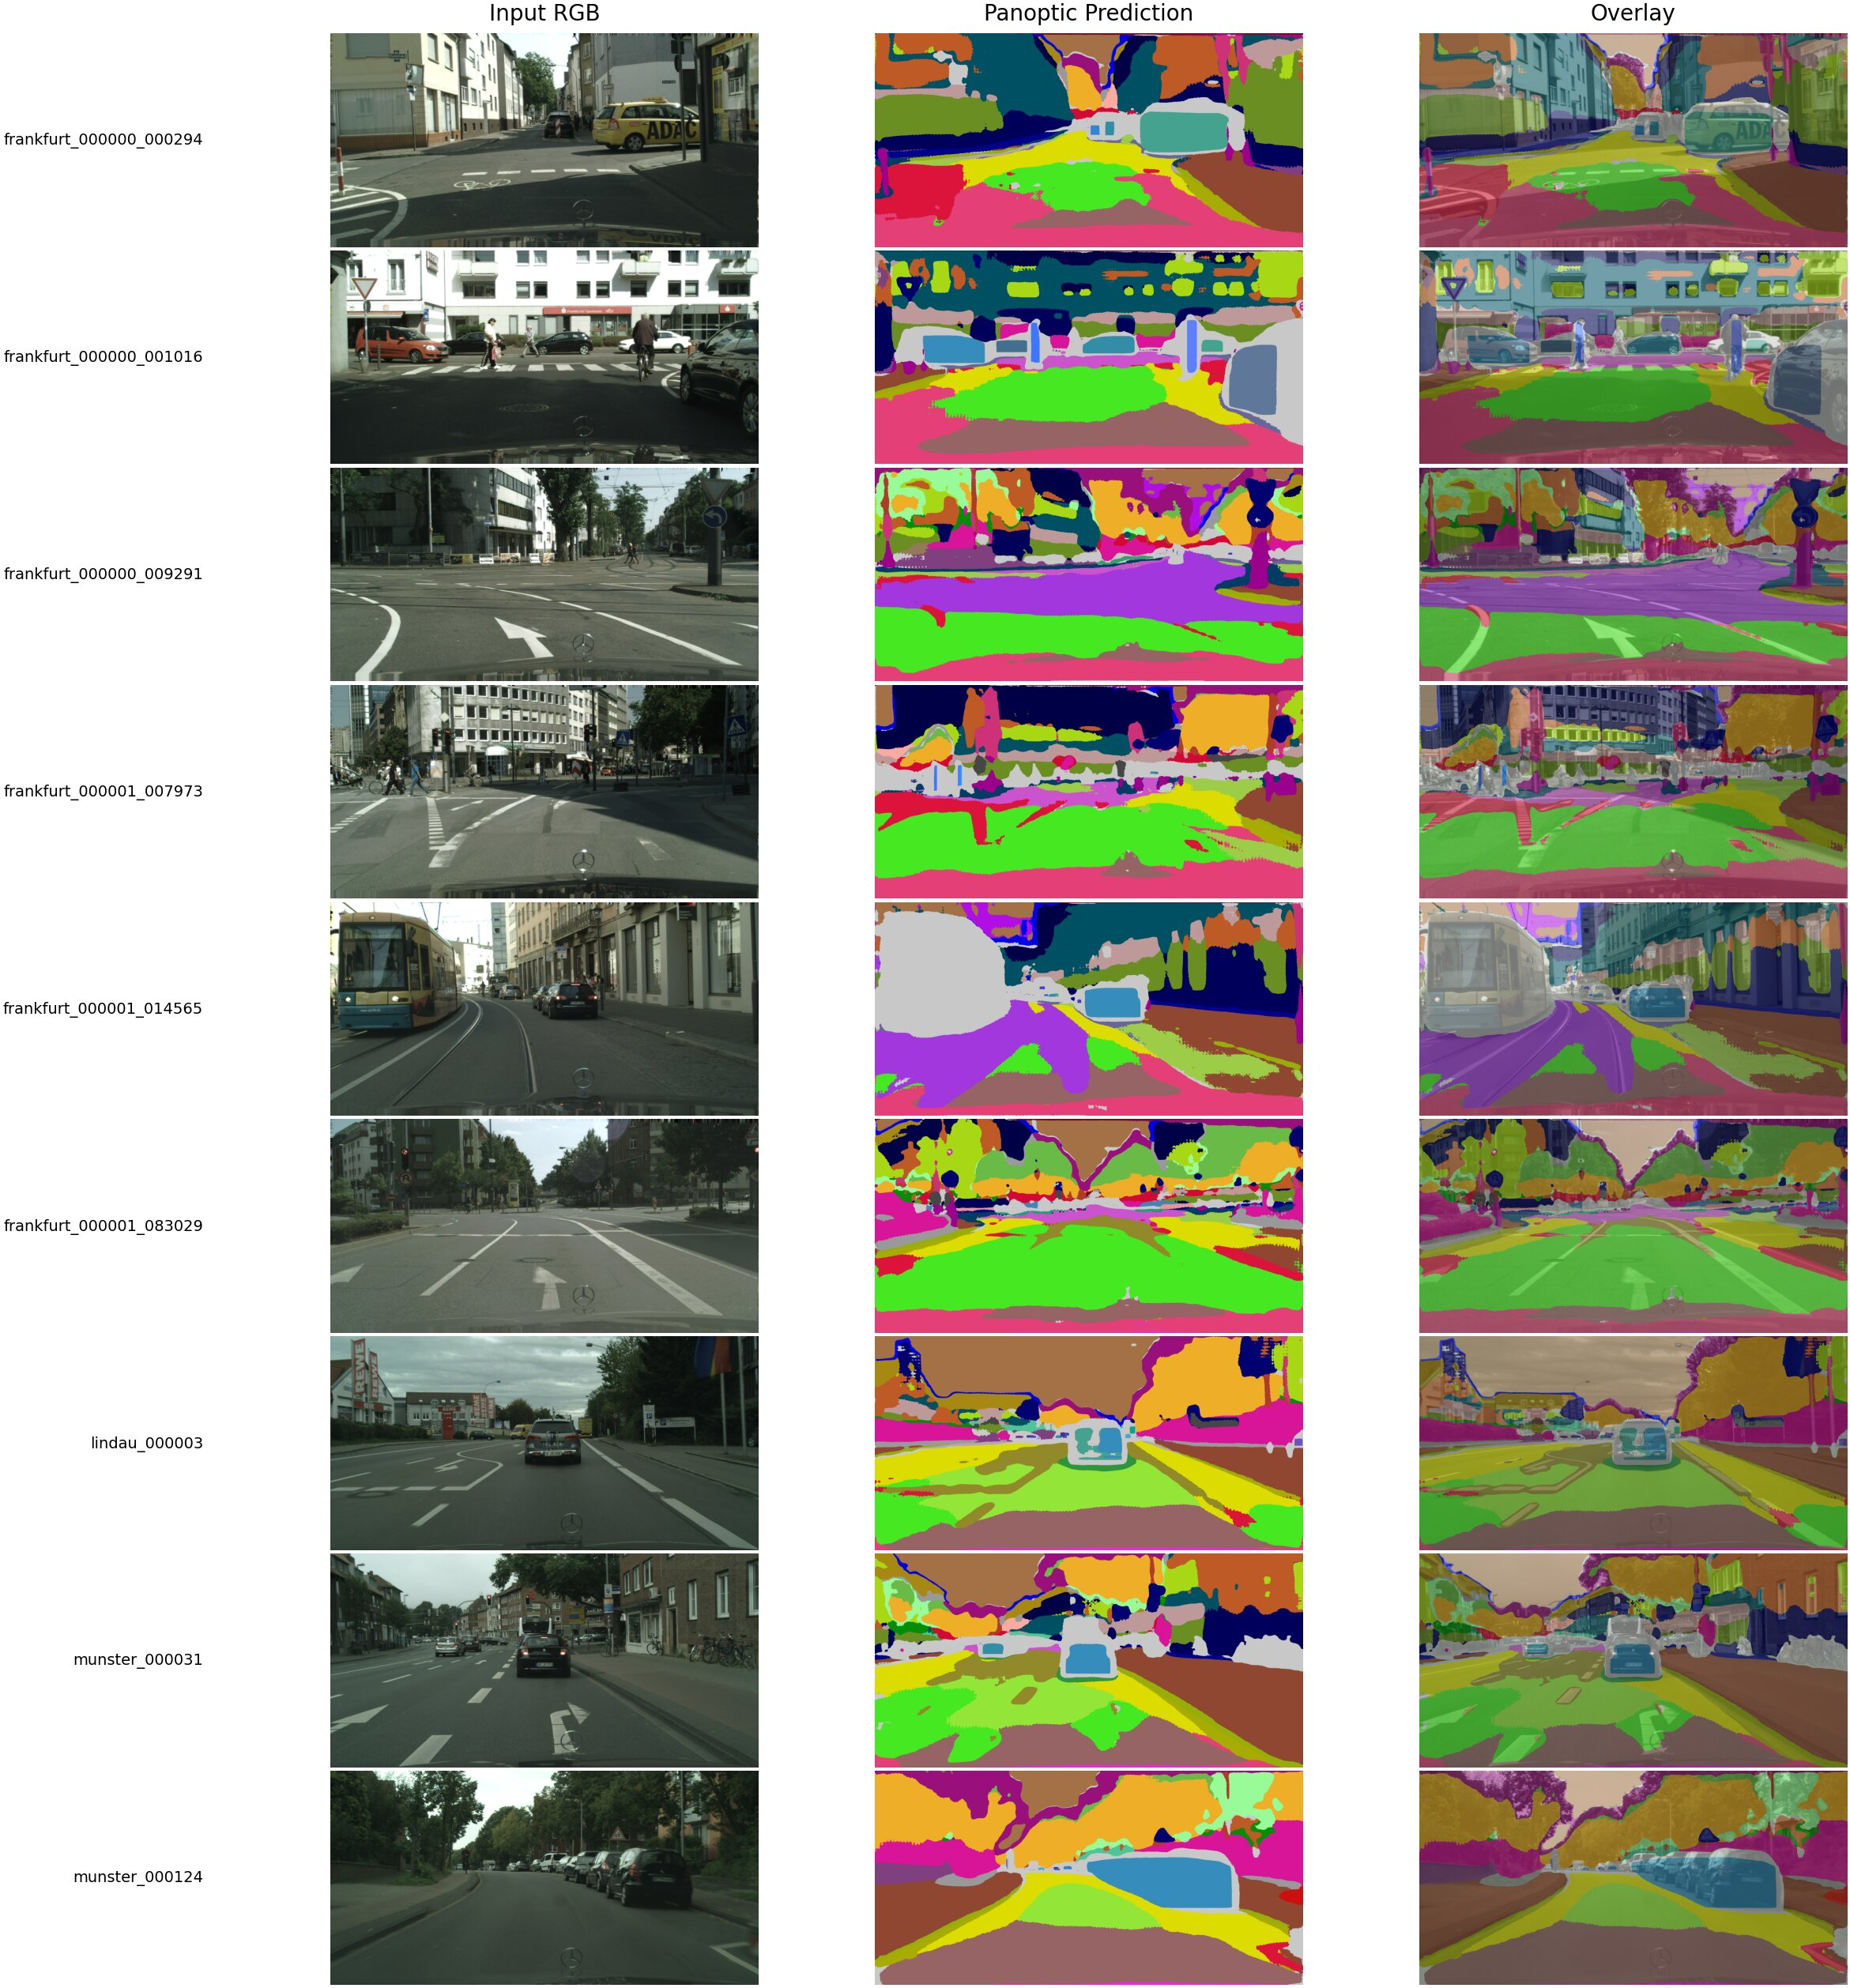
\includegraphics[width=0.92\linewidth]{figures/qualitative_stage3.jpg}
\caption{Stage-3 panoptic predictions on Cityscapes val (9 held-out images). Columns: RGB input, panoptic prediction in the $K=80$ pseudo-class space, RGB overlay ($\alpha{=}0.55$). Hungarian alignment to the 27-class Cityscapes evaluation taxonomy is computed only at metric time and is not applied here, so colors track pseudo-class IDs rather than benchmark classes. Light grey marks pixels that the network rejects below its semantic confidence threshold (void).}
\label{fig:supp_qualitative_stage3}
\end{figure}

\clearpage

%=========================================================================
\section{Implementation Details}
\label{sec:supp:impl}
%=========================================================================

This appendix expands the abbreviated experimental setup of the main paper (Section~\ref{sec:exp:setup}) with the full hyperparameter, optimizer, augmentation, and hardware configuration used for every reported result. All operating hyperparameters were fixed before consulting Cityscapes annotations and were not retuned afterwards.

\subsection{Datasets and Evaluation Protocol}
\label{sec:supp:impl:data}

Pseudo-label generation and panoptic network training use only Cityscapes train~\cite{cordts2016cityscapes} (2{,}975 images, no annotations). Evaluation is on Cityscapes val (500 images) under the 27-class CAUSE~\cite{kim2024cause} pseudo-vocabulary with a Hungarian map to the 27-class Cityscapes label space (\texttt{NUM\_CLASSES=27} in the official CUPS protocol~\cite{hahn2025cups}). The 27-class evaluation taxonomy includes the 19 standard semantic-segmentation classes plus parking, rail track, guard rail, bridge, tunnel, polegroup, caravan, and trailer. Cross-dataset transfer follows the CUPS~\cite{hahn2025cups} protocol on KITTI~\cite{geiger2012kitti}, Waymo V2~\cite{sun2020waymo}, and Mapillary Vistas v2~\cite{neuhold2017mapillary}.

\subsection{Stage-1: Pseudo-Label Generation}
\label{sec:supp:impl:stage1}

\paragraph{Frozen priors.}
DINOv2 ViT-B/14~\cite{oquab2024dinov2} backbone (no fine-tuning) and CAUSE-TR head~\cite{kim2024cause} (frozen, 90-dimensional concept-clusterbook code).

\paragraph{DCFA training.}
Hidden width $h{=}384$, three-layer MLP with concatenated 106-D input (90-D code + 16-D sinusoidal depth), $\sim$225K (225,114) trainable parameters. Loss: depth-correlation term $+\,\lambda_p \mathcal{L}_\text{preserve}$ with $\lambda_p{=}20$. Optimizer: AdamW, learning rate $10^{-3}$, weight decay $10^{-4}$, 10K iterations, batch size 32 images, sampling 1024 pixels and 1024 pixel pairs per image. The preservation term anchors the residual update to identity at initialisation and is re-applied at every step. Wall-clock: $\approx 1$ hour on a single GTX 1080 Ti.

\paragraph{$k$-means over-clustering.}
$k{=}80$ centroids on L2-normalised DCFA-adjusted CAUSE-TR codes, fitted on the 2{,}975 Cityscapes train images using \texttt{scikit-learn} mini-batch $k$-means (batch 4096, 100 iterations, fixed random seed). Centroids are saved once and reused throughout the rest of the pipeline.

\paragraph{Instance branch.}
DepthPro~\cite{bochkovskii2024depthpro} monocular depth (frozen, no fine-tuning). $3\times3$ Sobel kernels, gradient threshold $\tau_d{=}0.20$, 8-neighbour connected components inside thing-eligible semantic regions, $A_\text{min}{=}1000$ pixel filter, three iterations of $3\times3$ dilation.

\paragraph{SIMCF.}
Feature similarity threshold $\tau_\text{sim}{=}0.85$, depth-implausibility multiplier $\eta{=}2.5$. Adjacent-proposal merging (Step~B) and depth-implausibility void rejection (Step~C) are applied in this order.

\subsection{Stage-2: Panoptic Bootstrapping}
\label{sec:supp:impl:stage2}

Cascade Mask R-CNN~\cite{cai2018cascade} with three cascade stages on a frozen DINOv3 ViT-B/16 backbone~\cite{simeoni2025dinov3} (no backbone fine-tuning). 8K optimizer steps, batch size 8 (4 per GPU), AdamW (lr $10^{-4}$, weight decay $0.05$, $\beta_1{=}0.9$, $\beta_2{=}0.999$), cosine schedule with 500-step linear warmup. Loss includes DropLoss~\cite{wang2023cutler} ($\lambda_\text{drop}{=}1.0$) and self-enhanced copy-paste augmentation. Augmentation: random horizontal flip, random scale jitter $[0.5, 2.0]$, random crop $1024\times1024$, copy-paste with probability 0.5, photometric jitter (brightness $\pm$0.2, contrast $\pm$0.2, saturation $\pm$0.2). Wall-clock: $\approx 12$ hours on $2\times$ NVIDIA GTX 1080 Ti with PyTorch DistributedDataParallel.

\subsection{Stage-3: EMA Self-Training}
\label{sec:supp:impl:stage3}

Three EMA self-training rounds, each 5K optimizer steps. EMA coefficient 0.999. Three-scale teacher (scales $\{0.75, 1.0, 1.25\}$) with class-aware confidence thresholding (foreground $0.4$, background $0.3$). Same augmentation pipeline as Stage-2; same optimizer family and learning-rate base ($5\times10^{-5}$ at the start of each round, cosine schedule per round). Wall-clock: $\approx 16$ hours total on $2\times$ GTX 1080 Ti.

\subsection{Hardware and Wall-Clock Budget}
\label{sec:supp:impl:hardware}

All training is performed on $2\times$ NVIDIA GTX 1080 Ti GPUs (consumer-grade, 11 GB VRAM each) with PyTorch DistributedDataParallel. Total compute footprint per pipeline run: Stage-1 generation $\approx 2$ GPU-hours, Stage-2 bootstrapping $\approx 24$ GPU-hours ($\approx 12$ wall-clock on 2 GPUs), Stage-3 self-training $\approx 32$ GPU-hours ($\approx 16$ wall-clock on 2 GPUs); aggregate $\approx 58$ GPU-hours. The pipeline is therefore feasible on consumer-grade hardware that lacks the calibrated stereo rigs and synchronized video required by CUPS~\cite{hahn2025cups} at pseudo-label time.

\subsection{The Over-Cluster-to-Concept Map $\phi$ Uses No Ground-Truth Labels}
\label{sec:supp:impl:phi}

The map $\phi : \{1, \dots, 80\} \to \{1, \dots, 27\}$ used by the instance branch (Section~\ref{sec:method:baseline}) and SIMCF (Algorithm~\ref{alg:simcf}) is constructed entirely from frozen, self-supervised features. We make this explicit because reviewers may, on a quick reading, conflate the ``27'' in CAUSE's concept vocabulary with the ``27'' in the Cityscapes evaluation taxonomy; these are distinct objects.

\paragraph{What $\phi$ maps between.}
The \emph{source} side of $\phi$ is the set of 80 $k$-means cluster centroids fitted on the DCFA-adjusted 90-D semantic codes of Cityscapes train (Section~\ref{sec:method:baseline}). The \emph{target} side of $\phi$ is the set of 27 concept prototypes that live inside the frozen CAUSE-TR head~\cite{kim2024cause}. CAUSE-TR was trained without any human annotation, on Cityscapes train images using only the self-supervised concept-coherence objective; its 27 concept prototypes are therefore an internally-discovered partition of the latent space, not a label space.

\paragraph{How $\phi$ is computed.}
For each $k \in \{1, \dots, 80\}$, $\phi(k) = \arg\min_{c \in \{1, \dots, 27\}} \|\mu_k - p_c\|_2$, where $\mu_k$ is the $k$-th $k$-means centroid and $p_c$ is the $c$-th CAUSE concept prototype, both in the 90-D code space. This is a deterministic nearest-centroid lookup that runs once at the end of $k$-means fitting. The thing/stuff partition over the 27 CAUSE concepts (8 thing categories, 19 stuff categories) is fixed by CAUSE-TR's pretraining and is read off the frozen head; it is not derived from Cityscapes ground truth.

\paragraph{Where ground-truth enters the pipeline.}
The only ground-truth-derived component anywhere in the pipeline is the Hungarian map between the 27 CAUSE concept prototypes and the 27 Cityscapes evaluation classes, computed once over the 500-image Cityscapes \emph{val} set at metric time (Section~\ref{sec:exp:setup}). This Hungarian map is used only to compute PQ/SQ/RQ and never feeds back into the Stage-1 generator $G$, the panoptic network $F$, or any of the operating hyperparameters $(\tau_d, \tau_\text{sim}, \eta, A_\text{min}, \lambda_p, k)$. The values of these hyperparameters were fixed before consulting any Cityscapes annotation.

\subsection{DCFA Loss Definitions}
\label{sec:supp:impl:dcfa_loss}

Let $\mathcal{U}$ denote the set of $|\mathcal{U}| = 1024$ pixels sampled per image and $\mathcal{P}$ the set of $|\mathcal{P}| = 1024$ pixel pairs sampled from $\mathcal{U}$. Then
\begin{align*}
\mathcal{L}_\text{corr} &= \tfrac{1}{|\mathcal{P}|}\!\!\sum_{(i,j)\in\mathcal{P}} \mathcal{K}_{\sigma_d}(D_i, D_j)\,\big(1 - \cos(\tilde z_i, \tilde z_j)\big), \\
\mathcal{L}_\text{preserve} &= \tfrac{1}{|\mathcal{U}|} \sum_{u \in \mathcal{U}} \|\tilde z_u - z_u\|_2^2,
\end{align*}
where $\mathcal{K}_{\sigma_d}$ is the DepthG~\cite{sick2024depthg} depth-similarity kernel with bandwidth $\sigma_d=0.5$. Both losses are averaged over the sampled set per image, then averaged over the minibatch.

\subsection{Reproducibility Notes}
\label{sec:supp:impl:repro}

All random seeds are fixed at the beginning of each stage (DCFA training seed $42$, $k$-means seed $0$, Stage-2/3 dataloader seed $42$). Implementation: Python 3.10, PyTorch 2.1, Detectron2 0.6, CUDA 11.8. Stage-1 pseudo-labels and Stage-2/3 checkpoints will be released alongside the code upon publication.

%=========================================================================
\section{SIMCF Threshold Sensitivity}
\label{sec:supp:simcf_sweep}
%=========================================================================

SIMCF exposes two thresholds: $\tau_\text{sim}$ for adjacent-proposal feature merging (Step~B) and $\eta$ for depth-implausibility void rejection (Step~C). To verify that SIMCF's contribution is not the product of threshold tuning, we sweep both $\pm{\sim}12\%$ around the paper setting and re-evaluate pseudo-label quality on the full Cityscapes train set ($N{=}2975$).

\begin{table}[H]
\caption{SIMCF threshold sensitivity at fixed depth instances ($\tau_d{=}0.20$, DepthPro). Pseudo-label PQ is computed on Cityscapes train under the CUPS~\cite{hahn2025cups} 27-class protocol.}
\label{tab:simcf_sensitivity}
\centering
\small
\setlength{\tabcolsep}{6pt}
\begin{tabular}{l c c c c c c}
\toprule
Setting & $\tau_\text{sim}$ & $\eta$ & PQ & SQ & RQ & mIoU \\
\midrule
tighter         & 0.75 & 2.0 & 25.98 & 58.79 & 34.55 & 56.08 \\
baseline (paper) & 0.85 & 2.5 & 25.87 & 58.38 & 34.83 & 56.17 \\
looser          & 0.95 & 3.0 & 25.27 & 57.63 & 34.10 & 56.22 \\
\bottomrule
\end{tabular}
\end{table}

\paragraph{Interpretation.}
Pseudo-label PQ varies within a 0.71-point band (25.27--25.98) across the sweep, smaller than the $+1.31$ PQ super-additive gap from either single component to Both reported in the main paper's Table~\ref{tab:components}. Tighter thresholds slightly improve PQ; looser thresholds degrade modestly. The mechanism is therefore robust to moderate threshold perturbation rather than tuned-on-test.

%=========================================================================
\section{Depth Model Ablation}
\label{sec:supp:depth}
%=========================================================================

We compared three monocular depth estimators (SPIdepth, Depth-Anything v3~\cite{lin2025da3}, DepthPro~\cite{bochkovskii2024depthpro}) under representative gradient thresholds at the Stage-1 pseudo-label level. The rows in Table~\ref{tab:depth} are not a single leaderboard: some use the raw $K{=}80$ semantic map and others use the DCFA semantic map. They are reported jointly to separate mask quality from recognition quality while choosing the training-data configuration.

\begin{table}[H]
\caption{Depth and threshold diagnostics with aggregate SQ/RQ on Cityscapes train pseudo-labels.}
\label{tab:depth}
\centering
\small
\setlength{\tabcolsep}{6pt}
\begin{tabular}{l l c c c c}
\toprule
Depth & Sem. & $\tau$ & PQ & SQ & RQ \\
\midrule
SPIdepth & raw $K$=80 & 0.20 & 26.74 & 71.88 & 31.41 \\
DA v3~\cite{lin2025da3} & raw $K$=80 & 0.03 & 27.37 & 73.44 & 35.66 \\
DA v3~\cite{lin2025da3} & DCFA & 0.20 & 26.44 & 61.37 & 35.83 \\
DepthPro~\cite{bochkovskii2024depthpro} & DCFA & 0.01 & 27.81 & 63.07 & 37.40 \\
DepthPro~\cite{bochkovskii2024depthpro} & DCFA & 0.20 & 26.13 & 60.63 & 35.80 \\
\bottomrule
\end{tabular}
\end{table}

\paragraph{Discussion.}
The table shows why PQ alone is not a sufficient diagnostic for the depth branch. The sharper $\tau{=}0.01$ DepthPro setting has stronger standalone PQ/SQ/RQ, but it produces a fragmented training set with roughly 57 instances per image and more than half below 1000 pixels. The $\tau{=}0.20$ setting has lower standalone PQ but produces larger training targets, roughly 22 instances per image, which is the configuration used for panoptic bootstrapping. DA v3 at the same training-data threshold reaches a similar RQ, indicating that the choice is governed by the training signal produced by the depth branch rather than by the stuff/thing aggregate split.

%=========================================================================
\section{Out-of-Distribution Sanity Checks}
\label{sec:supp:ood}
%=========================================================================

The main paper reports cross-dataset transfer on three driving-scene benchmarks (KITTI~\cite{geiger2012kitti}, Waymo V2~\cite{sun2020waymo}, Mapillary v2~\cite{neuhold2017mapillary} in Section~\ref{sec:exp:generalization}) where the Cityscapes-derived pseudo-label vocabulary is in-domain. We additionally run two out-of-distribution sanity checks: (i) MOTS~\cite{voigtlaender2019mots} as a thing-only label space whose vocabulary is a subset of Cityscapes-things, and (ii) COCO-Stuff-27~\cite{caesar2018coco} as a vocabulary-mismatched object-centric dataset whose 27 classes overlap only partially with Cityscapes-27. Table~\ref{tab:cocooo} reports the result.

\begin{table}[H]
\caption{Out-of-distribution sanity checks on a thing-only label space (MOTS) and a vocabulary-mismatched object-centric dataset (COCO-Stuff-27). All numbers are percentages.}
\label{tab:cocooo}
\centering
\footnotesize
\setlength{\tabcolsep}{6pt}
\begin{tabular}{l c c c c}
\toprule
Dataset (OOD) & \# img & PQ & SQ & RQ \\
\midrule
MOTS~\cite{voigtlaender2019mots} thing-only & 2{,}862 & 61.10 & 88.71 & 65.80 \\
\quad CUPS~\cite{hahn2025cups} ref. & --- & 86.4 & 86.4 & 76.9 \\
COCO-Stuff-27~\cite{caesar2018coco} vocab.\ mismatch & 1{,}000 & \phantom{0}7.83 & 38.55 & 10.06 \\
\bottomrule
\end{tabular}
\end{table}

\paragraph{Interpretation.}
The MOTS result (61.10 PQ, SQ 88.71) confirms that mask geometry generalizes to a thing-only OOD vocabulary: the Stage-3 network produces high-quality masks on KITTI-style sequences even when the label space drops from 27 classes to a thing-only subset. The gap to the CUPS~\cite{hahn2025cups} reference (86.4 PQ) is recognition-driven (RQ 65.80 vs.\ 76.9) and reflects vocabulary granularity rather than a transfer failure of the architecture. The COCO-Stuff-27 result (7.83 PQ) is dominated by categories absent from a Cityscapes-derived pseudo-label space: most COCO-Stuff-27 categories (e.g.\ kitchenware, sports gear, food) have no analog in the Cityscapes pseudo-vocabulary and are unrecoverable by Hungarian alignment alone. This is the vocabulary boundary of in-domain training and not a transfer failure of the architecture; resolving it would require expanding the pseudo-label generator's vocabulary at training time, which is orthogonal to the contributions of this paper.

%=========================================================================
\section{Per-Class Cityscapes Metrics}
\label{sec:supp:perclass}
%=========================================================================

Table~\ref{tab:perclass} reports per-class PQ/SQ/RQ for the final trained network of the main paper (Section~\ref{sec:exp:main}) under the CUPS~\cite{hahn2025cups} 27-class evaluation protocol with Hungarian matching from the $K{=}80$ pseudo-vocabulary to the 27-class Cityscapes label space.

\begin{table}[H]
\caption{Per-class Cityscapes validation metrics for the final trained network. Values are percentages. Six classes (parking, guard rail, tunnel, polegroup, caravan, trailer) are vocabulary-dead; the twenty active classes carry the 35.83 PQ aggregate reported in the main paper.}
\label{tab:perclass}
\centering
\small
\setlength{\tabcolsep}{6pt}
\resizebox{\textwidth}{!}{%
\begin{tabular}{l c c c l c c c l c c c}
\toprule
Class & PQ & SQ & RQ & Class & PQ & SQ & RQ & Class & PQ & SQ & RQ \\
\midrule
road & 93.0 & 95.0 & 97.9 & tunnel & 0.0 & 0.0 & 0.0 & rider & 22.9 & 62.6 & 36.6 \\
sidewalk & 62.4 & 78.5 & 79.5 & pole & 2.0 & 72.3 & 2.8 & car & 70.7 & 88.7 & 79.7 \\
parking & 0.0 & 0.0 & 0.0 & polegroup & 0.0 & 0.0 & 0.0 & truck & 62.6 & 83.8 & 74.7 \\
rail track & 8.4 & 67.2 & 12.5 & traffic light & 6.2 & 60.3 & 10.3 & bus & 76.7 & 90.8 & 84.4 \\
building & 83.5 & 85.7 & 97.5 & traffic sign & 37.2 & 65.9 & 56.4 & caravan & 0.0 & 0.0 & 0.0 \\
wall & 32.3 & 67.7 & 47.8 & vegetation & 84.7 & 85.7 & 98.8 & trailer & 0.0 & 0.0 & 0.0 \\
fence & 20.3 & 63.0 & 32.1 & terrain & 35.7 & 73.4 & 48.6 & train & 77.2 & 88.7 & 87.0 \\
guard rail & 0.0 & 0.0 & 0.0 & sky & 86.1 & 89.9 & 95.7 & motorcycle & 0.1 & 100.0 & 0.1 \\
bridge & 17.2 & 64.5 & 26.7 & person & 13.4 & 71.4 & 18.7 & bicycle & 39.0 & 77.2 & 50.5 \\
\bottomrule
\end{tabular}
}
\end{table}

\paragraph{Discussion.}
Twenty active classes carry the 35.83 PQ aggregate. Large stuff regions (road 93.0, sky 86.1, vegetation 84.7, building 83.5) and large vehicles (car 70.7, bus 76.7, train 77.2) score above 70 PQ, since frozen semantic codes produce coherent regions and depth boundaries align with object extent. The remaining seven classes are vocabulary-coverage cases: parking, guard rail, tunnel, polegroup, caravan, and trailer lie outside the standard Cityscapes-19 panoptic benchmark and receive few positive examples in the $K{=}80$ over-cluster vocabulary, while motorcycle matches a single near-perfect instance (SQ$=$100). These cases reflect a property of the pseudo-label vocabulary rather than the network architecture, and their effect on the aggregate is bounded: removing them and averaging only over the standard Cityscapes-19 panoptic classes raises the protocol comparability of our headline.

The per-class table also exposes the recognition bottleneck for closely-spaced object classes: person reaches SQ$=$71.4 and rider SQ$=$62.6 (both above the 60-point band that classifies the per-class match as geometrically correct), while their RQ values (18.7 and 36.6 respectively) are recognition-limited by depth-based instance separation on co-planar pedestrian crowds. This is the failure mode discussed in the main paper's Conclusion (Section~\ref{sec:conclusion}).

\paragraph{SIMCF feature-merge diagnostics.}
Two qualitative metrics from the feature-guided merge step (Step~B) of SIMCF complete the picture. Average pseudo-instance count per image drops from 44 before the merge to 22 after, median instance size grows from 5{,}502 to 14{,}965 pixels, and stuff contamination falls from 50.7\% to 28.0\%. Many depth gradients are intra-object surface changes rather than object boundaries, and merging fragments whose semantic identity and dense appearance agree recovers the single-object structure that monocular depth had over-fragmented.

%=========================================================================
\section{Broader Impact}
\label{sec:impact}
%=========================================================================

\noindent Removing stereo and motion requirements at pseudo-label time broadens the range of imagery to which scene-centric unsupervised panoptic segmentation can be applied. The intended beneficiaries are autonomous-driving and robotic-perception pipelines that ingest monocular footage from phones, dashcams, or fixed cameras, where calibrated stereo rigs and synchronized video are unavailable.

The same property creates dual-use risk. A monocular-only pipeline lowers the data and hardware bar for deployment in surveillance and behavioral-monitoring settings that the original stereo-based methods could not easily reach. We do not release pretrained weights tuned to specific surveillance contexts, and the system as evaluated targets street-scene categories rather than person re-identification.

Two technical-bias concerns also follow from the design. First, the frozen pseudo-label vocabulary inherits any class-imbalance and dataset-bias signal already present in CAUSE-TR's~\cite{kim2024cause} Cityscapes-derived clusterbook; six dead classes, discussed in the main paper's limitations section, are a direct symptom and would compound on demographically less-represented scenes. Second, depth-based instance separation degrades on co-planar pedestrian crowds, which are over-represented in dense urban settings and may correlate with population density or geography. These limitations should be accounted for before downstream deployment, particularly in settings where the consequences of mispredicted person-class instances are non-trivial.

\end{document}
